\chapter{Misiones}\label{dept:Misiones}
\mapaparaguai{8}{Misiones}
\vfill\clearpage
\clearpage
\subsection*{Análise Temática por Distrito}
\addcontentsline{toc}{subsection}{Análise Temática por Distrito}

Os mapas a seguir mostram, para cada distrito de Misiones, o GSS final (pontuação geral), o risco social (criminalidade e instabilidade) e o potencial de autossuficiência (solo, água e energia). Cada valor é o calculado na metodologia GSS deste guia.

\begin{figure}[htbp]
\centering
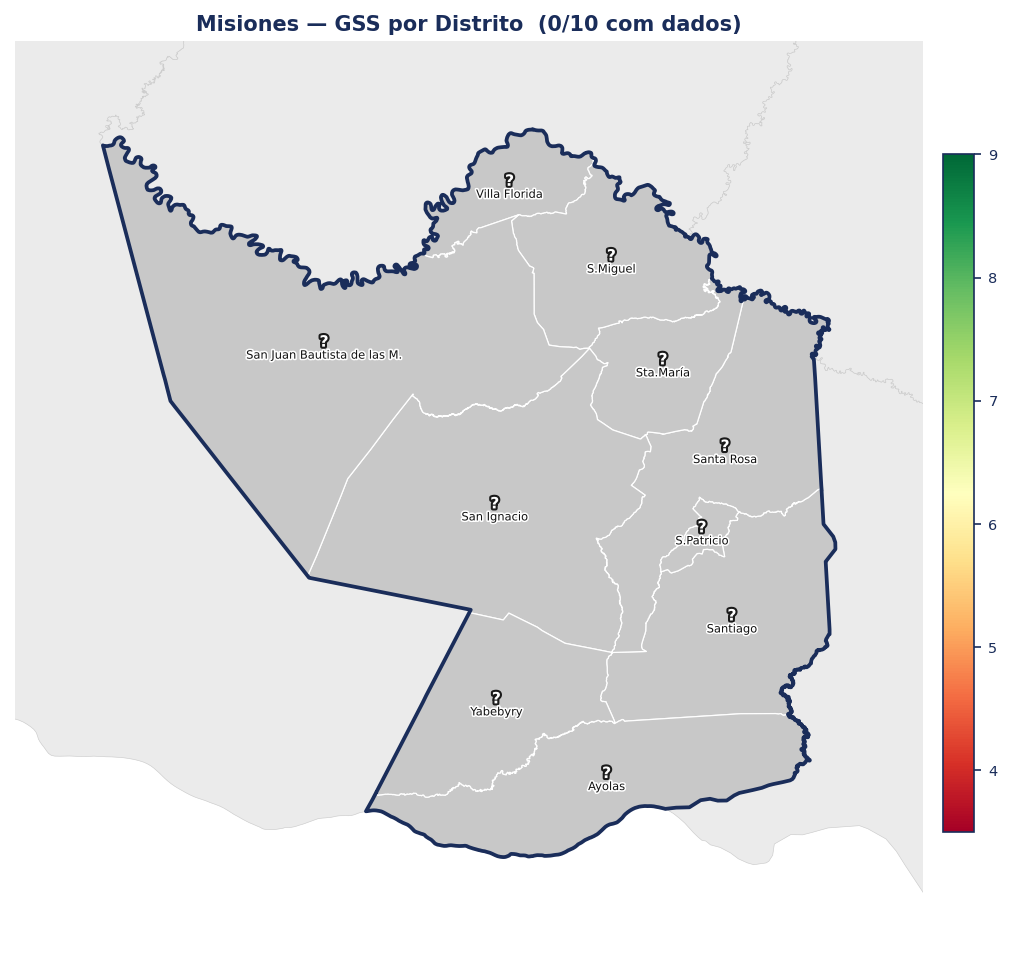
\includegraphics[width=\textwidth, height=0.55\textheight, keepaspectratio]{mapas/mapas_tematicos_dept_08_gss.png}
\caption{GSS (Global Safety Score) por distrito de Misiones. Verde = alta viabilidade · Vermelho = baixa viabilidade.}
\label{fig:gss-08}
\end{figure}

\vspace{0.5em}

\begin{figure}[htbp]
\centering
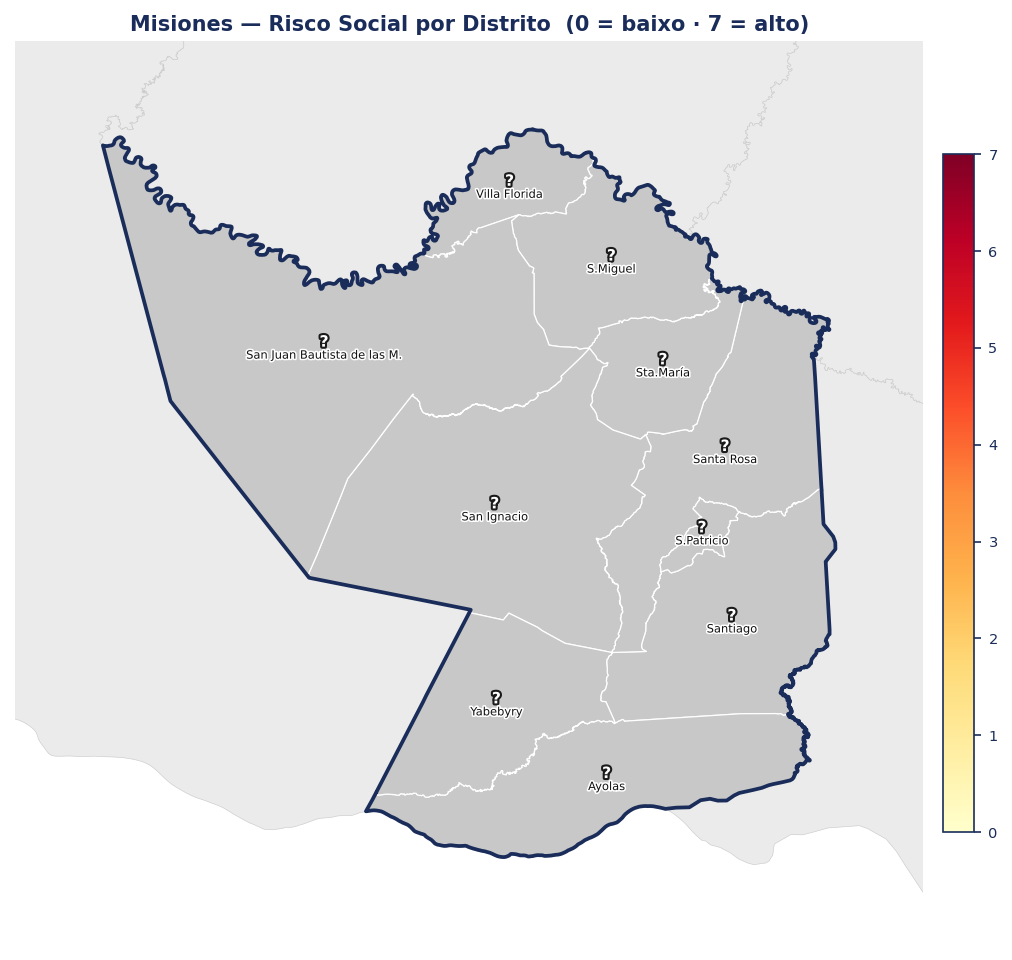
\includegraphics[width=\textwidth, height=0.55\textheight, keepaspectratio]{mapas/mapas_tematicos_dept_08_risco.png}
\caption{Risco social por distrito de Misiones. Amarelo = baixo risco · Vermelho = alto risco.}
\label{fig:risco-08}
\end{figure}

\clearpage

\begin{figure}[htbp]
\centering
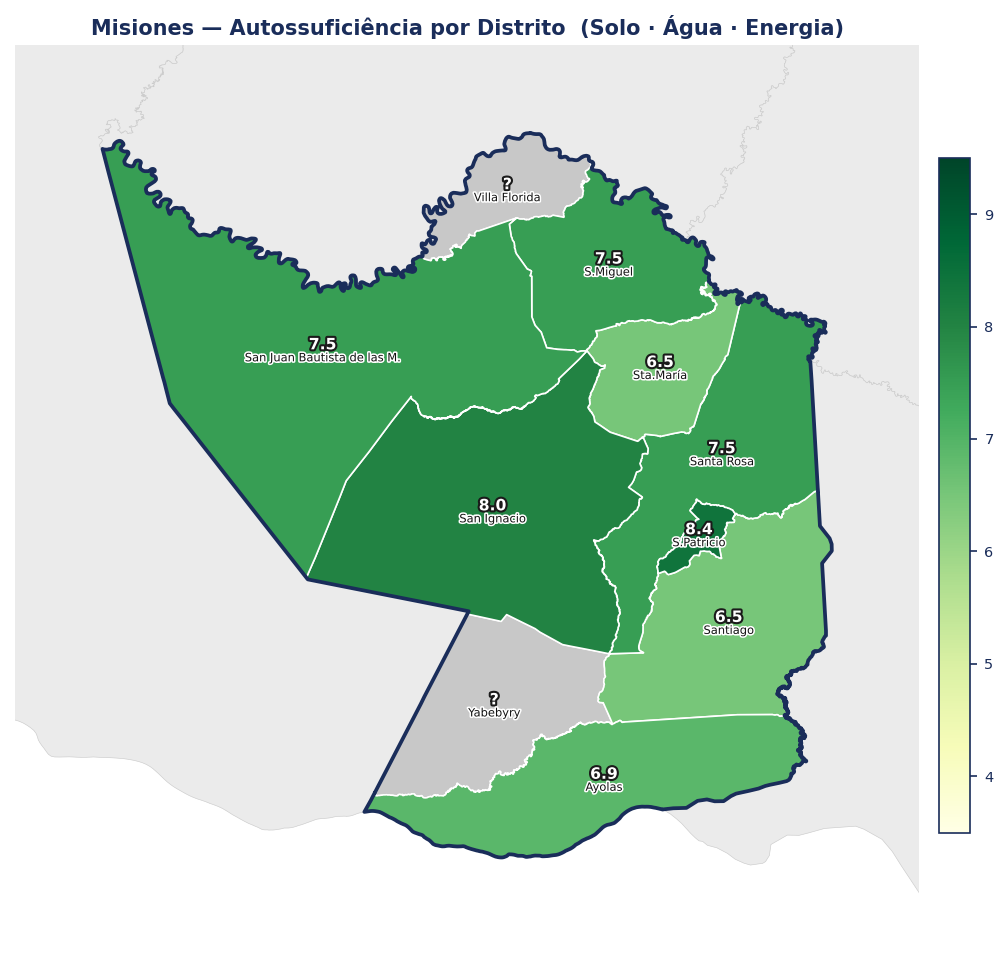
\includegraphics[width=\textwidth, height=0.55\textheight, keepaspectratio]{mapas/mapas_tematicos_dept_08_autosuf.png}
\caption{Autossuficiência por distrito de Misiones: solo, recursos hídricos e potencial energético. Branco = baixo · Verde escuro = alto.}
\label{fig:autosuf-08}
\end{figure}

\clearpage

\section{Misiones}

base agropecuaria (pecuaria, arroz, soja, mel) com polos urbanos em San
Ignacio, San Juan Bautista e Ayolas.

\subsection{Ficha climática de San Juan Bautista (capital
departamental)}

\textbf{Irradiância solar global --- (kWh/\allowbreak m²/\allowbreak dia):}


\begin{center}
\resizebox{\linewidth}{!}{%
{\renewcommand{\arraystretch}{1.2}%
\begin{tabular}{@{}c|c|c|c|c|c|c|c|c|c|c|c@{}}
\toprule
Jan & Fev & Mar & Abr & Mai & Jun & Jul & Ago & Set & Out & Nov & Dez \\
\midrule
6.72 & 6.24 & 5.35 & 4.27 & 3.26 & 2.73 & 3.11 & 3.77 & 4.48 & 5.37 &
6.41 & 6.79 \\
\bottomrule
\end{tabular}}%
}
\end{center}


Média anual: 4.87 kWh/\allowbreak m²/\allowbreak dia. Inclinação recomendada: 27° Norte (anual);
37° inverno; 17° verão.

\textbf{Precipitação --- (mm/\allowbreak mês):}


\begin{center}
\resizebox{\linewidth}{!}{%
{\renewcommand{\arraystretch}{1.2}%
\begin{tabular}{@{}c|c|c|c|c|c|c|c|c|c|c|c@{}}
\toprule
Jan & Fev & Mar & Abr & Mai & Jun & Jul & Ago & Set & Out & Nov & Dez \\
\midrule
136 & 119 & 133 & 164 & 143 & 88 & 72 & 62 & 93 & 181 & 184 & 168 \\
\bottomrule
\end{tabular}}%
}
\end{center}


Média anual: \textasciitilde1.545 mm/\allowbreak ano. Estação chuvosa Out-Nov; seca
Jul-Ago.
\clearpage
\subsection*{Dados Departamentais}

\subsection*{Segurança Pública}

\begin{tabularx}{\linewidth}{lX}
\toprule
Indicador & Valor \\
\midrule
Taxa de homicídios (por 100k hab) & ~2--4 (estimativa, abaixo da média nacional) \\
Crimes registrados (total/ano) & --- dados não desagregados publicamente \\
Número de comisarías & ~8 (estimativa departamental) \\
Índice segurança relativo & alto \\
\bottomrule
\end{tabularx}

Misiones é um dos departamentos mais tranquilos do Paraguai em termos de segurança pública. O Ministerio Público registra que o departamento responde por apenas \textbf{1\% das causas de homicídio doloso} nacional (2019--2024) --- proporção muito baixa e compatível com sua pequena população (cerca de 1,7\% do total nacional).

O departamento faz fronteira com Itapúa ao sul e com Ñeembucú a sudoeste, e está situado entre os rios Tebicuary e Paraná. Embora a fronteira sul com Argentina represente potencialmente uma rota de contrabando, o InSight Crime identifica o trecho Itapúa-Misiones como área de cruzamento, mas não Misiones como epicentro de violência. San Juan Bautista, capital departamental, é uma cidade pequena e tranquila.

A criminalidade é predominantemente de baixa intensidade, com crimes patrimoniais esporádicos. A baixa densidade populacional e o caráter rural do departamento contribuem para a baixa taxa de violência.

\subsection*{IDH e Desenvolvimento Humano}

\begin{tabularx}{\linewidth}{lX}
\toprule
Indicador & Valor \\
\midrule
IDH & 0,712 \\
Classificação IDH & alto \\
Ranking nacional (1=melhor) & 7/18 (empate estimado com Caaguazú) \\
Esperança de vida & 73,2 anos \\
Anos de escolaridade média & 8,3 anos \\
RNB per capita (USD PPA) & 8.900 \\
\bottomrule
\end{tabularx}

> Nota: IDH estimado com base no relatório PNUD 2020 e dados subnacionais da Global Data Lab para a região sul do Paraguai. Misiones tem perfil agropecuário consolidado e é o menor departamento em população da Região Oriental.

\begin{tabularx}{\linewidth}{lX}
\toprule
Indicador & Valor \\
\midrule
Taxa de pobreza total (\%) & 26,4\% \\
Taxa de pobreza extrema (\%) & 5,9\% \\
Índice de Gini & 0,442 \\
\bottomrule
\end{tabularx}

> Fonte: INE --- EPHC 2023 (dado de pobreza 26,4\% para Misiones conforme dados regionais Sul). Departamento com pobreza moderada para os padrões paraguaios.

\begin{tabularx}{\linewidth}{lX}
\toprule
Indicador & Valor \\
\midrule
Acesso a água potável (\%) & 80,3\% \\
Acesso a saneamento (\%) & 78,9\% \\
\bottomrule
\end{tabularx}

> Estimativa baseada em dados do Censo 2022 e perfil semiurbano/rural do departamento. San Juan Bautista, capital, tem boa infraestrutura para cidade de porte pequeno.

Misiones é o menor departamento em população da Região Oriental com IDH alto (0,712) e economia baseada em pecuária, agricultura e turismo histórico (Ruínas Jesuíticas). San Juan Bautista, a capital, é uma cidade tranquila com bons serviços básicos para seu tamanho. Para brasileiros, o departamento representa uma opção de vida rural com qualidade, distante dos centros urbanos. O turismo em torno das Missões Jesuíticas (San Cosme y Damián, Santa Rosa) oferece oportunidades de empreendimento. A pobreza de 26,4\% é moderada e o acesso a água (80,3\%) e saneamento (78,9\%) são satisfatórios. O departamento não tem grandes cidades, o que limita oportunidades de emprego formal mas reduz custos de vida. Indicado para quem busca tranquilidade rural, agronegócio ou turismo histórico-cultural.

\subsection*{Sistema Prisional}

{\small
{\small
\begin{tabularx}{\linewidth}{lXXXX}
\toprule
Nome & Município & Capacidade & População & Superlotação \\
\midrule
Penitenciaría Regional de San Juan Bautista & San Juan Bautista & 120 & ~210 & ~175\% \\
\bottomrule
\end{tabularx}
}
}

\begin{tabularx}{\linewidth}{lX}
\toprule
Indicador & Valor \\
\midrule
Total de estabelecimentos & 1 \\
Capacidade total (vagas) & ~120 \\
População carcerária total & ~210 \\
Taxa de superlotação & ~175\% \\
\% presos provisórios & ~65\% \\
\bottomrule
\end{tabularx}

Misiones é um dos departamentos menos populosos do Paraguai, com economia baseada em pecuária e agricultura. O único estabelecimento penal localiza-se em San Juan Bautista, capital departamental, e atende detentos de todos os 10 municípios do departamento.

O perfil de criminalidade em Misiones é relativamente baixo em comparação com departamentos de fronteira. O tráfico de gado e crimes contra a propriedade rural são as infrações mais comuns que alimentam a população carcerária local.

O departamento faz fronteira com a Argentina ao sul (rio Paraná), mas o volume de comércio e tráfego nessa fronteira é menor do que em Itapúa ou Alto Paraná, reduzindo a pressão do crime organizado transnacional.

\textbf{Para imigrantes:} Misiones é um departamento tranquilo e com baixo custo de vida. San Juan Bautista tem infraestrutura modesta mas funcional. O sistema prisional tem impacto mínimo na vida cotidiana da maioria dos municípios. Indicado para quem busca ambiente rural e tranquilo.

\subsection*{Recursos Hídricos Subterrâneos}

\begin{tabularx}{\linewidth}{lXXX}
\toprule
Aquífero & Cobertura no Dept. & Profundidade Média & Vazão Típica \\
\midrule
Guarani / Misiones (afloramento e confinado) & ~80\% & 60--250 m & 20--80 m$^3$/h \\
Aluvial (rio Tebicuary e afluentes) & Faixas ribeirinhas & 8--25 m & 5--15 m$^3$/h \\
\bottomrule
\end{tabularx}

\begin{tabularx}{\linewidth}{lX}
\toprule
Parâmetro & Valor \\
\midrule
Profundidade média --- Guarani (m) & 60--200 \\
Profundidade máxima recomendada (m) & 300 \\
Vazão típica (m$^3$/h) & 15--60 \\
Custo estimado perfuração (USD) & 2.500 -- 9.000 \\
Qualidade da água & boa a excelente \\
pH médio & 6,5--7,5 \\
Outorga necessária & sim \\
Órgão regulador & MADES --- DGPCRH \\
\bottomrule
\end{tabularx}

O departamento de Misiones dá nome à própria Formação Misiones, unidade geológica que compõe o Aquífero Guarani nesta região. Os afloramentos dessa formação são frequentes, com arenitos de alta permeabilidade que facilitam a recarga do sistema. As profundidades de captação são relativamente baixas (60--150 m), tornando a perfuração mais econômica que em outros departamentos. A água é de boa qualidade, com baixa mineralização, pH neutro e ausência de contaminantes naturais. Uso principal: abastecimento doméstico, pecuária e irrigação. San Juan Bautista (capital) tem rede pública do SENASA.

Misiones é um departamento com economia agropecuária forte e terrenos acessíveis. O Aquífero Guarani é amplamente disponível em profundidades relativamente rasas (60--150 m), o que reduz o custo de perfuração para USD 2.500--7.000. Excelente para propriedades rurais com uso doméstico e irrigação. A rede pública cobre apenas centros urbanos. Poço artesiano é a solução padrão e economicamente vantajosa para qualquer imóvel rural. Licença do MADES obrigatória.

\subsection*{Aptidão do Solo}

\begin{tabularx}{\linewidth}{lXX}
\toprule
Tipo de Solo & \% do Território & Características \\
\midrule
Ultissolos / Planossolos (Alfissolos) & 40\% & Solos com horizonte B argiloso-imperfeito; limitações físicas para agricultura intensiva \\
Entissolos arenosos (Quartzarênicos) & 30\% & Solos derivados de arenito, baixa fertilidade natural, suscetíveis à erosão e seca \\
Oxissolos (Latossolos) & 15\% & Solos basálticos no nordeste do departamento, melhor aptidão agrícola \\
Inceptissolos / Aluviais & 15\% & Planícies do Rio Paraguai e Rio Pilcomayo; solos jovens de boa fertilidade \\
\bottomrule
\end{tabularx}

\begin{tabularx}{\linewidth}{lXX}
\toprule
Classe & \% Território & Uso Recomendado \\
\midrule
Lavoura intensiva & 15\% & Soja e milho nas áreas basálticas do nordeste \\
Lavoura extensiva & 25\% & Mandioca, sorgo, girassol, amendoim \\
Pastagem natural/melhorada & 40\% & Pecuária extensiva e semi-intensiva (atividade principal) \\
Floresta / reserva & 15\% & Remanescentes nativos, matas ciliares \\
Sem aptidão agrícola & 5\% & Áreas alagáveis, urbanas, degradadas \\
\bottomrule
\end{tabularx}

\begin{tabularx}{\linewidth}{lX}
\toprule
Parâmetro & Valor \\
\midrule
pH médio & 5,0 -- 6,5 \\
Fertilidade natural & média \\
Teor de matéria orgânica & médio \\
Necessidade de calcário & parcial \\
\bottomrule
\end{tabularx}

Misiones não é o destino prioritário para imigrantes brasileiros com foco em agricultura de grãos em larga escala. A vocação do departamento é predominantemente pecuária extensiva. Para quem busca pecuária de corte, a região oferece boas condições naturais de pastagem e clima adequado. As áreas com solos basálticos no nordeste têm potencial para soja, mas são relativamente restritas. O custo da terra é moderado. Comparativamente aos solos do Brasil, as limitações físico-hídricas de Misiones o colocam abaixo da média dos solos paranaenses.

\subsection*{Terra Rural}

\begin{tabularx}{\linewidth}{lXXX}
\toprule
Tipo & Preço (USD/ha) & Faixa & Tendência \\
\midrule
Agrícola alta produtividade & 4.500 & 3.000 -- 6.500 & $\uparrow$ \\
Pastagem & 2.200 & 1.500 -- 3.200 & $\uparrow$ \\
Mata / reserva & 900 & 500 -- 1.500 & $\rightarrow$ \\
\bottomrule
\end{tabularx}

\begin{tabularx}{\linewidth}{lX}
\toprule
Parâmetro & Valor \\
\midrule
Valorização anual média (\%) & 5--7\% \\
Lote mínimo rural (ha) & 20 \\
Imposto territorial rural (\%) & 1\% sobre valor fiscal \\
Liquidez do mercado & média \\
\bottomrule
\end{tabularx}

\begin{tabularx}{\linewidth}{lXXX}
\toprule
Indicador & Misiones (PY) & Rio Grande do Sul (BR) & Mato Grosso do Sul (BR) \\
\midrule
Terra agrícola (USD/ha) & 3.000--6.500 & 12.000--22.000 & 10.000--20.000 \\
Terra pastagem (USD/ha) & 1.500--3.200 & 5.000--9.000 & 4.000--8.000 \\
Custo relativo & ~28\% do RS & referência RS & referência MS \\
\bottomrule
\end{tabularx}

Misiones é um departamento com vocação pecuária e turística. Os preços de terra são competitivos, especialmente em zonas de pastagem para gado de corte.

\subsection*{Mercado Imobiliário}

\textbf{Capital:} San Juan Bautista

\begin{tabularx}{\linewidth}{lXX}
\toprule
Tipo & Preço (USD/m$^2$) & Aluguel (USD/mês) \\
\midrule
Apartamento 2 quartos & 500 -- 800 & 180 -- 350 \\
Casa 3 quartos & 420 -- 700 & 160 -- 320 \\
\bottomrule
\end{tabularx}

\begin{tabularx}{\linewidth}{lX}
\toprule
Parâmetro & Valor \\
\midrule
Valorização anual (\%) & 4--6\% \\
Disponibilidade de financiamento & limitada (cooperativas e BNF) \\
Bairros mais valorizados & Centro, proximidades do Parque Industrial, bairros residenciais com infraestrutura de Yacyretá \\
\bottomrule
\end{tabularx}

\textbf{Vale a pena comprar ou alugar?}
San Juan Bautista é uma cidade de porte moderado (aprox. 50.000 hab.) com boa qualidade de vida para padrões paraguaios. A presença da Usina Yacyretá cria uma infraestrutura de serviços acima da média regional. Para quem atua na agroindústria ou pecuária regional, compra de casa é vantajosa.

\textbf{Áreas recomendadas:}
San Juan Bautista, capital departamental, é a única cidade com mercado imobiliário minimamente organizado em Misiones. Concentre-se em imóveis próximos ao centro, onde a infraestrutura é melhor e a liquidez, ainda que baixa, é maior.

\textbf{Armadilhas comuns:}
O mercado é muito pequeno e poucos imóveis são comercializados formalmente, o que dificulta a precificação e aumenta o risco de pagar acima do valor de mercado. Consulte mais de um corretor local e, se possível, contrate avaliador independente para embasar qualquer oferta de compra.

\subsection*{Cobertura Celular}

{\small
{\small
\begin{tabularx}{\linewidth}{lXXXXX}
\toprule
Operadora & 2G & 3G & 4G & 5G & Cobertura Pop. \\
\midrule
Tigo & 82\% & 72\% & 60\% & --- & 76\% \\
Personal/Claro & 75\% & 65\% & 52\% & --- & 70\% \\
VOX & 45\% & 30\% & 15\% & --- & 38\% \\
\bottomrule
\end{tabularx}
}
}

> \textbf{Nota:} Misiones é um departamento pequeno com população relativamente concentrada na capital San Juan Bautista e ao longo da Ruta 1 (Asunción--Encarnación). A Ruta 1 garante boa cobertura linear; interior mais afastado tem sinal reduzido.

\begin{tabularx}{\linewidth}{lX}
\toprule
Parâmetro & Valor \\
\midrule
Melhor operadora rural & Tigo \\
Velocidade 4G média (Mbps) & 15--35 \\
Áreas sem cobertura & Interior oeste, margens do rio Paraguai, zonas de mata \\
Sinal em propriedade rural & moderado \\
\bottomrule
\end{tabularx}

\begin{tabularx}{\linewidth}{lXXX}
\toprule
Plano & Operadora & USD/mês & Dados \\
\midrule
Pré-pago básico (7 dias) & Tigo & ~2,50 & 3 GB \\
Pré-pago intermediário (30 dias) & Personal & ~5,00 & 8 GB \\
Pós-pago entrada & Tigo & ~12,00 & 15 GB + chamadas \\
Pós-pago intermediário & Personal/Claro & ~18,00 & 30 GB + chamadas \\
\bottomrule
\end{tabularx}

\subsection*{Internet}

\begin{tabularx}{\linewidth}{lX}
\toprule
Indicador & Valor \\
\midrule
\% população com internet & ~62\% \\
\% com banda larga fixa & ~18\% dos domicílios \\
Velocidade média download (Mbps) & 20--50 (urbano) / 4--12 (rural) \\
Velocidade média upload (Mbps) & 8--18 (urbano) \\
\bottomrule
\end{tabularx}

\begin{tabularx}{\linewidth}{lXX}
\toprule
Tecnologia & Disponibilidade & Velocidade Típica \\
\midrule
Fibra ótica (FTTH) & San Juan Bautista, San Ignacio & 30--200 Mbps \\
Cabo HFC & San Juan Bautista & 20--100 Mbps \\
Rádio/Wireless & Municípios ao longo da Ruta 1 & 5--40 Mbps \\
ADSL (Copaco) & Interior & 1--8 Mbps \\
Satélite (Starlink) & Todo o departamento & 50--200 Mbps \\
\bottomrule
\end{tabularx}

\begin{tabularx}{\linewidth}{lXXX}
\toprule
Provedor & Tecnologia & Área de cobertura & Preço ref. (USD/mês) \\
\midrule
Tigo & Fibra/Rádio & San Juan Bautista + municípios da Ruta 1 & 18--45 \\
Claro/Personal & Fibra/Rádio & San Juan Bautista & 15--40 \\
Copaco & ADSL/Rádio & Interior & 10--25 \\
Starlink & Satélite LEO & Todo o departamento & ~44 + equip. ~370 \\
\bottomrule
\end{tabularx}

A cobertura rural de Misiones é \textbf{moderada} ao longo da Ruta 1, e \textbf{limitada} no interior oeste:

\clearpage
\newpage
\secaoDiagnostico{Ayolas}{\mapaDistrito{0802}}{Ayolas é uma cidade planejada construída para dar suporte à Usina
Hidrelétrica de Yacyretá, às margens do Lago de mesmo nome, na fronteira
com a Argentina. Única no Paraguai por seu projeto urbano ordenado e pela
sua identidade econômica singular, consolidou-se como a \textbf{``Capital
Mundial da Pesca do Dourado''}, atraindo turistas de todo o continente.
Para o imigrante brasileiro, representa uma opção incomum: infraestrutura
urbana acima da média regional, lazer à beira do lago e a possibilidade
de renda no setor de serviços ligado ao turismo de pesca esportiva e à
própria usina binacional.

\subsubsection{Recomendação
Técnica}

Indicada para perfis que buscam qualidade de vida em ambiente
semi-urbano, com destaque para aposentados e famílias que valorizam lazer
aquático e boa infraestrutura. O entorno do lago e a dependência da rota
sul impõem atenção logística. GSS 6,9 reflete o equilíbrio entre boa
infraestrutura e exposição hídrica intrínseca ao lago. Referência atual
de score: GSS 6,9.

}
\begin{table}[ht!]
\small \begin{tabular}{p{3.0cm}p{0.8cm}p{6.0cm}} \toprule
\textbf{Critério} & \textbf{Nota} & \textbf{Justificativa} \\ \midrule
A - Ameaças Estratégicas & 6,0 & Cidade planejada e isolada; baixa visibilidade estratégica militar; distância de centros de poder \\
B - Risco Social & 7,0 & ~25.000 hab. com perfil diverso (funcionários da usina, pescadores, turistas); coesão social razoável \\
C - Riscos Naturais & 6,5 & Risco hídrico intrínseco ao lago Yacyretá; variações de nível podem afetar áreas ribeirinhas \\
D - Autossuficiência & 7,5 & Hospital regional; comércio diversificado; pesca abundante; mercado de serviços ativo \\
E - Institucional & 7,5 & Presença institucional da binacional Yacyretá; serviços públicos de qualidade acima da média regional \\
\midrule
 \textbf{GSS FINAL} & \textbf{6,9} & \textbf{Moderadamente Seguro (boa opção para aposentados e perfis de serviços; requer autonomia logística).} \\ \bottomrule
 \end{tabular}
\end{table}
\subsubsection{Vulnerabilidades e
Mitigação}\label{vuln-ayolas-0802}

\begin{itemize}
\tightlist
\item
  \textbf{Dependência da Rota Sul:} A única via de acesso asfáltica pelo
  sul (PY01 / ramal) pode ser comprometida em cheias do Paraná
  (Mitigação: embarcação própria ou mapeamento de rotas alternativas via
  San Juan Bautista; estoque de 14 dias de suprimentos).
\item
  \textbf{Variação do Lago:} Flutuações do nível do reservatório podem
  afetar imóveis ribeirinhos e embarques (Mitigação: escolher terrenos
  acima da cota de inundação histórica; consultar dados da EBY).
\item
  \textbf{Economia Sazonal:} Receita turística concentrada na temporada
  de pesca (abr--set) gera variação de demanda por serviços
  (Mitigação: diversificar renda com serviços à usina ou produção
  alimentar local).
\item
  \textbf{Infraestrutura Dependente da Usina:} Fornecimento elétrico
  privilegiado, mas centralizado (Mitigação: sistema solar off-grid de
  backup com autonomia mínima de 72h).
\end{itemize}

\subsubsection{Dossiê de Campo}\label{dossie-ayolas-0802}
\begin{description}[style=nextline,leftmargin=0.5cm,font=\bfseries]
\item[Coordenadas]  27°23'S 56°51'W.
\item[Topografia]  Relevo plano a levemente ondulado à margem do Lago Yacyretá. Altitude \textasciitilde 80m. Área de \textasciitilde 1.200 km². Zona de planície aluvial; risco sísmico desprezível.
\item[Alvos Estratégicos]  Usina Hidrelétrica de Yacyretá (binacional Paraguai-Argentina); porto fluvial; infraestrutura turística de pesca esportiva. Cidade planejada com baixíssima densidade industrial estratégica.
\item[Fallout]  Ventos predominantes do Norte (NE). Baixo risco de fallout direto.
\item[População]  \textasciitilde25.000 habitantes (est. 2024). Cidade planejada com perfil misto: funcionários da usina, prestadores de serviços, pescadores profissionais e turistas.
\item[Densidade]  \textasciitilde 20 hab/\allowbreak km² (núcleo urbano concentrado; entorno rural pouco habitado).
\item[Vias de Acesso]  Rota departamental pavimentada conectando à PY01 em San Patricio (\textasciitilde 45 km) e a San Juan Bautista (\textasciitilde 111 km). Acesso fluvial pelo Lago Yacyretá.
\item[Serviços]  Hospital Regional de Ayolas (referência sub-regional); banco; supermercados; escolas de ensino médio; marinas e infraestrutura hoteleira de porte acima da média regional.
\item[Custo de Vida]  Médio; levemente superior ao interior de Misiones pela demanda turística, mas abaixo de Encarnación.
\item[Preço da Terra]  US\$ 2.000--3.500/\allowbreak ha (áreas rurais arredores); US\$ 500--900/\allowbreak m² (imóvel urbano com vista para o lago). Aluguéis: USD 200--350/\allowbreak mês para 2 quartos.
\item[Hidrologia]  Lago Yacyretá (reservatório do Rio Paraná). Risco de variação de nível gerenciado pela EBY. Poços artesianos disponíveis no entorno.
\item[Clima]  Subtropical Úmido. Verões muito quentes (amenizados pela brisa do lago); invernos amenos com geadas raras. Precipitação: \textasciitilde1.586 mm/\allowbreak ano.
\item[Energia]  Fornecimento prioritário e de alta qualidade derivado da própria Yacyretá. Maior estabilidade elétrica da região sul.
\item[Água]  Rede municipal consolidada abastecida pelo lago; qualidade tratada adequada.
\item[Qualidade do Solo]  Solo arenoso-argiloso de aptidão média; mais indicado para pecuária leve e horticultura familiar do que para lavouras mecanizadas.
\item[Recursos Locais]  Pesca esportiva e comercial (dourado, surubí, pacú); turismo náutico; produção de serviços para a usina; pecuária extensiva no entorno.
\item[Segurança]  Baixa criminalidade; presença policial adequada ao porte da cidade; comunidade pequena e coesa. Vigilância necessária em picos de temporada turística.
\item[Leis Local]  Cidade planejada sob regime especial vinculado à binacional Yacyretá. \\ \textbf{Livre de Restrição} de Fronteira (fora da faixa de 50 km da fronteira argentina). \\ \textit{Aquisição de terra rural: verificar restrições de zona de proteção do reservatório junto à EBY e INDERT.}
\end{description}
\textbf{Fonte climática:} NASA POWER Climatology API (período 2001-2020)

\textbf{Fonte luminosa:} estimativa world atlas

\paragraph{Irradiação Solar
(kWh/\allowbreak m²/\allowbreak dia)}


\begin{center}
\resizebox{\linewidth}{!}{%
{\renewcommand{\arraystretch}{1.2}%
\begin{tabular}{@{}c|c|c|c|c|c|c|c|c|c|c|c|c@{}}
\toprule
Jan & Fev & Mar & Abr & Mai & Jun & Jul & Ago & Set & Out & Nov & Dez & Média \\
\midrule
6.74 & 6.25 & 5.37 & 4.27 & 3.19 & 2.70 & 3.05 & 3.74 & 4.44 & 5.36 &
6.49 & 6.87 & \textbf{4.87} \\
\bottomrule
\end{tabular}}%
}
\end{center}


\textbf{Inclinação solar recomendada:} 27° N (anual) · 37° N (inverno
jun-ago) · 17° N (verão nov-jan)

\paragraph{Precipitação (mm/\allowbreak mês)}


\begin{center}
\resizebox{\linewidth}{!}{%
{\renewcommand{\arraystretch}{1.2}%
\begin{tabular}{@{}c|c|c|c|c|c|c|c|c|c|c|c|c@{}}
\toprule
Jan & Fev & Mar & Abr & Mai & Jun & Jul & Ago & Set & Out & Nov & Dez & Total/\allowbreak ano \\
\midrule
147 & 120 & 140 & 175 & 128 & 94 & 69 & 65 & 99 & 192 & 182 & 175 &
\textbf{1586 mm} \\
\bottomrule
\end{tabular}}%
}
\end{center}


\paragraph{Poluição Luminosa}

\begin{longtable}[]{@{}ll@{}}
\toprule\noalign{}
Parâmetro & Valor \\
\midrule\noalign{}
\endhead
\bottomrule\noalign{}
\endlastfoot
Escala Bortle & 3 --- Céu rural \\
Radiância artificial & 0.8 nW/\allowbreak cm²/\allowbreak sr \\
\end{longtable}
\paragraph{Solo (SoilGrids 2.0, média ponderada 0--30
cm)}

\begin{longtable}[]{@{}ll@{}}
\toprule\noalign{}
Parâmetro & Valor \\
\midrule\noalign{}
\endhead
\bottomrule\noalign{}
\endlastfoot
pH (H$_2$O) & 5.25 \\
Carbono orgânico (SOC) & 18.62 g/\allowbreak kg \\
Argila & 16.12 \% \\
Areia & 64.38 \% \\
Silte (calc.) & 19.5 \% \\
Densidade aparente & 1.37 g/\allowbreak cm³ \\
\textbf{Aptidão agrícola} & \textbf{Média} \\
\end{longtable}

\subsubsection{Indicadores Sociais}

\textbf{Fontes:} PNUD 2020, INE\footnote{\fineINE} Censo 2022, INE\footnote{\fineINE} EPHC 2023, Ministerio
Público 2024\\
\textbf{Nota:} Valores marcados como \emph{(dept.)} referem-se ao
departamento de Misiones; valores \emph{(dist.)} são específicos deste
distrito. Dados marcados \emph{(est.)} são estimativas.

\begin{longtable}[]{@{}
  >{\raggedright\arraybackslash}p{(\linewidth - 4\tabcolsep) * \real{0.4231}}
  >{\raggedright\arraybackslash}p{(\linewidth - 4\tabcolsep) * \real{0.2692}}
  >{\raggedright\arraybackslash}p{(\linewidth - 4\tabcolsep) * \real{0.3077}}@{}}
\toprule\noalign{}
\begin{minipage}[b]{\linewidth}\raggedright
Indicador
\end{minipage} & \begin{minipage}[b]{\linewidth}\raggedright
Valor
\end{minipage} & \begin{minipage}[b]{\linewidth}\raggedright
Âmbito
\end{minipage} \\
\midrule\noalign{}
\endhead
\bottomrule\noalign{}
\endlastfoot
IDH (2020) & 0,712 & dept. \\
Ranking IDH nacional & 7/\allowbreak 18 (empate estimado com Caaguazú) & dept. \\
Esperança de vida & 73,2 anos & dept. \\
Escolaridade média & 10.2 anos & dist. \\
RNB per capita (USD PPA) & 8.900 & dept. \\
Pobreza monetária (\%) & 26,4\% & dept. \\
Pobreza extrema (\%) & 5,9\% & dept. \\
Índice de Gini & 0,442 & dept. \\
Acesso a água potável (\%) & 80,3\% & dept. \\
Acesso a saneamento (\%) & 78,9\% & dept. \\
Taxa de homicídios (est., /\allowbreak 100k hab) & \textasciitilde2--4 (estimativa,
abaixo da média nacional) & dept. \\
Índice de segurança & alto & dept. \\
População (Censo 2022) & N/\allowbreak D & dist. \\
Idade mediana & N/\allowbreak D & dist. \\
Taxa de fecundidade & N/\allowbreak D & dist. \\
\end{longtable}
\subsubsection{Combustível}

\textbf{Referência:} PETROPAR /\allowbreak  postos locais (2024) \textbf{Tipo de
localidade:} Interior

\begin{longtable}[]{@{}lll@{}}
\toprule\noalign{}
Combustível & USD/\allowbreak litro & Gs/\allowbreak litro (aprox.) \\
\midrule\noalign{}
\endhead
\bottomrule\noalign{}
\endlastfoot
Gasolina 93 oct & 0.98 & 7,252 \\
Gasolina 97 oct (premium) & 1.08 & 7,992 \\
Diesel & 0.91 & 6,734 \\
\end{longtable}

\begin{quote}
Preços podem variar ±5\% conforme posto e sazonalidade. Chaco e interior
remoto apresentam maior variação.
\end{quote}

\subsubsection{Cobertura Celular}

\textbf{Fonte:} CONATEL PY /\allowbreak  operadoras (2024)

\begin{longtable}[]{@{}ll@{}}
\toprule\noalign{}
Parâmetro & Valor \\
\midrule\noalign{}
\endhead
\bottomrule\noalign{}
\endlastfoot
Cobertura 4G população (dept.) & 82\% \\
Cobertura 4G área rural & 62\% \\
Melhor operadora & Tigo \\
Qualidade rural & moderada \\
\end{longtable}

\begin{quote}
Para áreas rurais fora do núcleo urbano, recomenda-se chip Tigo como
principal e Personal como backup.
\end{quote}

\subsubsection{Internet}

\textbf{Fonte:} CONATEL /\allowbreak  Speedtest Ookla (2024)

\begin{longtable}[]{@{}ll@{}}
\toprule\noalign{}
Parâmetro & Valor \\
\midrule\noalign{}
\endhead
\bottomrule\noalign{}
\endlastfoot
Velocidade média download & 40 Mbps \\
Domicílios com internet (dept.) & 50\% \\
Tecnologia predominante & rádio \\
Opção rural & Starlink disponível (\textasciitilde USD 44/\allowbreak mês) \\
\end{longtable}

\subsubsection{Mercado Imobiliário e Terra
Rural}

\textbf{Fonte:} INDERT /\allowbreak  Clasificados.com.py (2024)

\begin{longtable}[]{@{}ll@{}}
\toprule\noalign{}
Tipo & Referência \\
\midrule\noalign{}
\endhead
\bottomrule\noalign{}
\endlastfoot
Terra agrícola alta prod. (USD/\allowbreak ha) & 4,000 \\
Imóvel urbano (USD/\allowbreak m²) & 600 \\
Aluguel 2 quartos (USD/\allowbreak mês) & 240 \\
\end{longtable}

\begin{quote}
Valores de referência departamental. Localidades menores podem ter
preços 20--40\% abaixo da capital departamental. \#\#\# Saúde
\end{quote}

\textbf{Fonte:} MSPBS /\allowbreak  IPS Paraguay (2024-2026), consolidação
departamental e proxy local

\begin{longtable}[]{@{}ll@{}}
\toprule\noalign{}
Serviço & Disponibilidade \\
\midrule\noalign{}
\endhead
\bottomrule\noalign{}
\endlastfoot
USF /\allowbreak  Posto de Saúde & sim \\
Hospital Regional & não \\
IPS (seguro social) & não \\
Farmácia & sim \\
Distância ao hospital de referência & \textasciitilde111 km (San Juan
Bautista) \\
\end{longtable}

\textbf{Principais estabelecimentos:} USF local; referencia hospitalar
em San Juan Bautista

\textbf{Observação para imigrantes:} Atendimento primario local ou em
raio curto; casos de maior complexidade seguem para San Juan Bautista.
Cobertura privada continua recomendada para especialidades e urgências
de maior complexidade.
\newpage
\secaoDiagnostico{San Ignacio}{\mapaDistrito{0803}}{San Ignacio Guazú é o motor comercial e logístico de Misiones. Oferece a
infraestrutura de serviços e suprimentos mais robusta da região,
garantindo uma capacidade de geração de recursos (proteína e grãos) de
nível superior. Contudo, seu papel geográfico como o principal nó
rodoviário do Sul a torna vulnerável em cenários de instabilidade,
exigindo um posicionamento rural periférico para mitigar os riscos da
visibilidade estratégica.

\subsubsection{Recomendação
Técnica}

Altamente indicado como centro de operações, logística ou para
residências rurais a média distância do centro (15-20 km). Requer um
planejamento de segurança focado na proteção contra fluxos migratórios e
bloqueios de estrada. O GSS de 6.7 reflete a solidez dos recursos e da
segurança institucional da região. Referência atual de score: GSS 6.7.

}
\begin{table}[ht!]
\small \begin{tabular}{p{3.0cm}p{0.8cm}p{6.0cm}} \toprule
\textbf{Critério} & \textbf{Nota} & \textbf{Justificativa} \\ \midrule
A - Ameaças Estratégicas & 5.0 & Nó logístico tático vital no Sul; alvo estratégico de alta visibilidade e controle \\
B - Risco Social & 6.0 & Maior população regional e densidade urbana significativa; risco social em crises \\
C - Riscos Naturais & 7.0 & Geologia muito estável e baixo risco de desastres naturais graves \\
D - Autossuficiência & 8.0 & Recursos agropecuários excepcionais: gado de elite, arroz, soja e água abundante \\
E - Institucional & 7.5 & Forte segurança institucional e serviços de saúde de referência departamental \\
\midrule
 \textbf{GSS FINAL} & \textbf{6.7} & \textbf{Moderadamente Seguro (Ideal como base administrativa e de suprimentos para o Sul do país).} \\ \bottomrule
 \end{tabular}
\end{table}
\subsubsection{Vulnerabilidades e
Mitigação}\label{vuln-san-ignacio-0803}

\begin{itemize}
\tightlist
\item
  \textbf{Funil Logístico:} O controle do cruzamento PY01/\allowbreak PY04 pode
  isolar o tráfego regional (Mitigação: residência rural afastada 10-15
  km do eixo asfáltico, com rotas de terra alternativas mapeadas).
\item
  \textbf{Pressão de Massa:} Alvo provável de convergência de refugiados
  em crises urbanas nacionais (Mitigação: estabelecimento de base com
  fortificação física e autonomia total).
\item
  \textbf{Dependência de Redes:} Alta dependência de sistemas
  centralizados para comércio (Mitigação: poço artesiano próprio e
  sistema solar off-grid).
\end{itemize}

\subsubsection{Dossiê de Campo}\label{dossie-san-ignacio-0803}
\begin{description}[style=nextline,leftmargin=0.5cm,font=\bfseries]
\item[Coordenadas]  26°53'S 57°01'W.
\item[Topografia]  Relevo predominantemente plano a suavemente ondulado, solo de alta fertilidade. Altitude \textasciitilde 135m. Área vasta de \textasciitilde 2.026 km². Geologicamente muito estável, risco sísmico desprezível (zona intraplaca).
\item[Alvos Estratégicos]  Nó Logístico Vital do Sul (Cruzamento das Rutas PY01 e PY04); Polo comercial e financeiro do departamento; Terminais de carga e silos; Patrimônio histórico jesuítico massivo. Ausência de bases militares de grande porte, mas centro de gravidade populacional e de suprimentos.
\item[Fallout]  Ventos predominantes do Norte (NE) e Leste. Baixo risco de fallout direto.
\item[População]  29.430 habitantes (Censo 2022 Final). É o distrito mais populoso de Misiones. Perfil urbano-rural dinâmico.
\item[Densidade]  \textasciitilde 14,5 hab/\allowbreak km² (Baixa densidade no total, mas com núcleo urbano denso, indicando vulnerabilidade social urbana em crises agudas).
\item[Vias de Acesso]  Ponto nevrálgico. Conecta Assunção (225 km), Encarnación e Pilar. Infraestrutura asfáltica de alta qualidade. Risco extremo de saturação rodoviária por fluxos migratórios em cenários de ruptura metropolitana ou internacional.
\item[Serviços]  Melhor infraestrutura comercial e bancária do departamento. Hospital Distrital e forte rede de clínicas privadas. Polo educacional universitário.
\item[Custo de Vida]  Médio-baixo; economia movimentada pelo agronegócio e serviços.
\item[Preço da Terra]  US\$ 4.000-6.500/\allowbreak ha (áreas agrícolas mecanizadas); US\$ 1.500-2.500/\allowbreak ha (áreas de pecuária extensiva em campos baixos).
\item[Hidrologia]  Diversos arroios locais tributários do Rio Tebicuary. Baixo risco de inundações sistêmicas catastróficas no núcleo urbano (cota segura). Risco de isolamento de acessos rurais em chuvas extremas (>1.600 mm/\allowbreak ano).
\item[Clima]  Subtropical Úmido. Verões quentes; invernos secos com geadas ocasionais.
\item[Energia]  Rede nacional (Itaipu/\allowbreak Yacyretá). Nodo central de distribuição elétrica regional com manutenção prioritária.
\item[Água]  Abundante via poços artesianos profundos e sistemas de junta de saneamento consolidados.
\item[Qualidade do Solo]  Solo franco-argiloso (vermelho) e solos hidromórficos nas baixadas; muito fértil e profundo, excelente para soja, arroz, milho e pastagens.
\item[Recursos Locais]  Coração da pecuária de elite e rizicultura. Produção massiva de gado de corte, arroz, soja e mel. Elevadíssimo potencial para autossuficiência e suprimento regional de longa duração.
\item[Segurança]  Cidade dinâmica com criminalidade urbana comum (furtos/\allowbreak roubos) em ascensão. Segurança institucional forte através da Polícia Nacional e tradição comunitária conservadora. Vigilância necessária contra abigeato em áreas rurais.
\item[Leis Local: Município histórico ("Capital do Barroco Hispano-Guarani"). Livre de Restrição de Fronteira]  Fora da faixa de 50km da fronteira argentina.
\end{description}
\textbf{Fonte climática:} NASA POWER Climatology API (período 2001-2020)

\textbf{Fonte luminosa:} estimativa world atlas

\paragraph{Irradiação Solar
(kWh/\allowbreak m²/\allowbreak dia)}


\begin{center}
\resizebox{\linewidth}{!}{%
{\renewcommand{\arraystretch}{1.2}%
\begin{tabular}{@{}c|c|c|c|c|c|c|c|c|c|c|c|c@{}}
\toprule
Jan & Fev & Mar & Abr & Mai & Jun & Jul & Ago & Set & Out & Nov & Dez & Média \\
\midrule
6.72 & 6.24 & 5.35 & 4.27 & 3.26 & 2.73 & 3.11 & 3.77 & 4.48 & 5.37 &
6.41 & 6.79 & \textbf{4.87} \\
\bottomrule
\end{tabular}}%
}
\end{center}


\textbf{Inclinação solar recomendada:} 27° N (anual) · 37° N (inverno
jun-ago) · 17° N (verão nov-jan)

\paragraph{Precipitação (mm/\allowbreak mês)}


\begin{center}
\resizebox{\linewidth}{!}{%
{\renewcommand{\arraystretch}{1.2}%
\begin{tabular}{@{}c|c|c|c|c|c|c|c|c|c|c|c|c@{}}
\toprule
Jan & Fev & Mar & Abr & Mai & Jun & Jul & Ago & Set & Out & Nov & Dez & Total/\allowbreak ano \\
\midrule
142 & 118 & 137 & 172 & 135 & 92 & 72 & 66 & 98 & 188 & 185 & 173 &
\textbf{1577 mm} \\
\bottomrule
\end{tabular}}%
}
\end{center}


\paragraph{Poluição Luminosa}

\begin{longtable}[]{@{}ll@{}}
\toprule\noalign{}
Parâmetro & Valor \\
\midrule\noalign{}
\endhead
\bottomrule\noalign{}
\endlastfoot
Escala Bortle & 3 --- Céu rural \\
Radiância artificial & 0.8 nW/\allowbreak cm²/\allowbreak sr \\
\end{longtable}
\paragraph{Solo (SoilGrids 2.0, média ponderada 0--30
cm)}

\begin{longtable}[]{@{}ll@{}}
\toprule\noalign{}
Parâmetro & Valor \\
\midrule\noalign{}
\endhead
\bottomrule\noalign{}
\endlastfoot
pH (H$_2$O) & 5.3 \\
Carbono orgânico (SOC) & 18.05 g/\allowbreak kg \\
Argila & 26.91 \% \\
Areia & 48.44 \% \\
Silte (calc.) & 24.7 \% \\
Densidade aparente & 1.38 g/\allowbreak cm³ \\
\textbf{Aptidão agrícola} & \textbf{Média} \\
\end{longtable}

\subsubsection{Indicadores Sociais}

\textbf{Fontes:} PNUD 2020, INE\footnote{\fineINE} Censo 2022, INE\footnote{\fineINE} EPHC 2023, Ministerio
Público 2024\\
\textbf{Nota:} Valores marcados como \emph{(dept.)} referem-se ao
departamento de Misiones; valores \emph{(dist.)} são específicos deste
distrito. Dados marcados \emph{(est.)} são estimativas.

\begin{longtable}[]{@{}
  >{\raggedright\arraybackslash}p{(\linewidth - 4\tabcolsep) * \real{0.4231}}
  >{\raggedright\arraybackslash}p{(\linewidth - 4\tabcolsep) * \real{0.2692}}
  >{\raggedright\arraybackslash}p{(\linewidth - 4\tabcolsep) * \real{0.3077}}@{}}
\toprule\noalign{}
\begin{minipage}[b]{\linewidth}\raggedright
Indicador
\end{minipage} & \begin{minipage}[b]{\linewidth}\raggedright
Valor
\end{minipage} & \begin{minipage}[b]{\linewidth}\raggedright
Âmbito
\end{minipage} \\
\midrule\noalign{}
\endhead
\bottomrule\noalign{}
\endlastfoot
IDH (2020) & 0,712 & dept. \\
Ranking IDH nacional & 7/\allowbreak 18 (empate estimado com Caaguazú) & dept. \\
Esperança de vida & 73,2 anos & dept. \\
Escolaridade média & 9.9 anos & dist. \\
RNB per capita (USD PPA) & 8.900 & dept. \\
Pobreza monetária (\%) & 26,4\% & dept. \\
Pobreza extrema (\%) & 5,9\% & dept. \\
Índice de Gini & 0,442 & dept. \\
Acesso a água potável (\%) & 80,3\% & dept. \\
Acesso a saneamento (\%) & 78,9\% & dept. \\
Taxa de homicídios (est., /\allowbreak 100k hab) & \textasciitilde2--4 (estimativa,
abaixo da média nacional) & dept. \\
Índice de segurança & alto & dept. \\
População (Censo 2022) & 29.430 habitantes & dist. \\
Idade mediana & N/\allowbreak D & dist. \\
Taxa de fecundidade & N/\allowbreak D & dist. \\
\end{longtable}
\subsubsection{Combustível}

\textbf{Referência:} PETROPAR /\allowbreak  postos locais (2024) \textbf{Tipo de
localidade:} Interior

\begin{longtable}[]{@{}lll@{}}
\toprule\noalign{}
Combustível & USD/\allowbreak litro & Gs/\allowbreak litro (aprox.) \\
\midrule\noalign{}
\endhead
\bottomrule\noalign{}
\endlastfoot
Gasolina 93 oct & 0.98 & 7,252 \\
Gasolina 97 oct (premium) & 1.08 & 7,992 \\
Diesel & 0.91 & 6,734 \\
\end{longtable}

\begin{quote}
Preços podem variar ±5\% conforme posto e sazonalidade. Chaco e interior
remoto apresentam maior variação.
\end{quote}

\subsubsection{Cobertura Celular}

\textbf{Fonte:} CONATEL PY /\allowbreak  operadoras (2024)

\begin{longtable}[]{@{}ll@{}}
\toprule\noalign{}
Parâmetro & Valor \\
\midrule\noalign{}
\endhead
\bottomrule\noalign{}
\endlastfoot
Cobertura 4G população (dept.) & 82\% \\
Cobertura 4G área rural & 62\% \\
Melhor operadora & Tigo \\
Qualidade rural & moderada \\
\end{longtable}

\begin{quote}
Para áreas rurais fora do núcleo urbano, recomenda-se chip Tigo como
principal e Personal como backup.
\end{quote}

\subsubsection{Internet}

\textbf{Fonte:} CONATEL /\allowbreak  Speedtest Ookla (2024)

\begin{longtable}[]{@{}ll@{}}
\toprule\noalign{}
Parâmetro & Valor \\
\midrule\noalign{}
\endhead
\bottomrule\noalign{}
\endlastfoot
Velocidade média download & 40 Mbps \\
Domicílios com internet (dept.) & 50\% \\
Tecnologia predominante & rádio \\
Opção rural & Starlink disponível (\textasciitilde USD 44/\allowbreak mês) \\
\end{longtable}

\subsubsection{Mercado Imobiliário e Terra
Rural}

\textbf{Fonte:} INDERT /\allowbreak  Clasificados.com.py (2024)

\begin{longtable}[]{@{}ll@{}}
\toprule\noalign{}
Tipo & Referência \\
\midrule\noalign{}
\endhead
\bottomrule\noalign{}
\endlastfoot
Terra agrícola alta prod. (USD/\allowbreak ha) & 4,000 \\
Imóvel urbano (USD/\allowbreak m²) & 600 \\
Aluguel 2 quartos (USD/\allowbreak mês) & 240 \\
\end{longtable}

\begin{quote}
Valores de referência departamental. Localidades menores podem ter
preços 20--40\% abaixo da capital departamental. \#\#\# Saúde
\end{quote}

\textbf{Fonte:} MSPBS /\allowbreak  IPS Paraguay (2024-2026), consolidação
departamental e proxy local

\begin{longtable}[]{@{}ll@{}}
\toprule\noalign{}
Serviço & Disponibilidade \\
\midrule\noalign{}
\endhead
\bottomrule\noalign{}
\endlastfoot
USF /\allowbreak  Posto de Saúde & sim \\
Hospital Regional & sim \\
IPS (seguro social) & não \\
Farmácia & sim \\
Distância ao hospital de referência & \textasciitilde45 km (San Juan
Bautista) \\
\end{longtable}

\textbf{Principais estabelecimentos:} USF local; referencia hospitalar
em San Juan Bautista

\textbf{Observação para imigrantes:} Atendimento primario local ou em
raio curto; casos de maior complexidade seguem para San Juan Bautista.
Cobertura privada continua recomendada para especialidades e urgências
de maior complexidade.
\newpage
\secaoDiagnostico{San Juan Bautista}{\mapaDistrito{0801}}{San Juan Bautista é o bastião da estabilidade e tradição em Misiones.
Oferece a melhor combinação de segurança institucional (apoio militar e
policial) e vastidão territorial de Itapúa/\allowbreak Misiones. Sua força reside na
excepcional qualidade de seus recursos hídricos e na solidez de sua base
pecuária de elite. É o local ideal para quem busca proximidade com
serviços estatais e de saúde de referência, mantendo-se em um ambiente
de baixíssima densidade demográfica e alta coesão social.

\subsubsection{Recomendação
Técnica}

Altamente indicado como base logística, administrativa ou residencial
rural de alto padrão. O GSS de 6.9 reflete a excepcional estabilidade
institucional e a riqueza de recursos da localidade. Referência atual de
score: GSS 6.9.

}
\begin{table}[ht!]
\small \begin{tabular}{p{3.0cm}p{0.8cm}p{6.0cm}} \toprule
\textbf{Critério} & \textbf{Nota} & \textbf{Justificativa} \\ \midrule
A - Ameaças Estratégicas & 6.5 & Capital departamental e base militar estratégica; alvo tático mas com alta proteção estatal \\
B - Risco Social & 7.5 & Baixíssima densidade demográfica total e população pequena; excelente segurança social \\
C - Riscos Naturais & 7.0 & Geologia muito estável e baixo risco de desastres naturais graves \\
D - Autossuficiência & 7.5 & Recursos agropecuários excepcionais: berço do gado de elite, abundância hídrica e solo fértil \\
E - Institucional & 8.5 & Altíssima segurança institucional e melhor suporte estatal do departamento \\
\midrule
 \textbf{GSS FINAL} & \textbf{7.4} & \textbf{Seguro (Localidade de elite para quem busca suporte institucional e recursos de alta qualidade).} \\ \bottomrule
 \end{tabular}
\end{table}
\subsubsection{Vulnerabilidades e
Mitigação}\label{vuln-san-juan-bautista-0801}

\begin{itemize}
\tightlist
\item
  \textbf{Visibilidade Administrativa:} Alvo burocrático em crises
  políticas nacionais (Mitigação: residência rural afastada 10-15 km do
  núcleo urbano governamental).
\item
  \textbf{Dependência de Rodovias:} O bloqueio da PY01 atinge a
  logística de suprimentos industriais (Mitigação: aproveitar a base de
  pecuária local para autonomia alimentar e manter rotas vicinais
  mapeadas).
\item
  \textbf{Instabilidade Pluvial:} Vulnerabilidade de culturas de
  sequeiro (Mitigação: investimento em irrigação a partir de poços
  profundos).
\end{itemize}

\subsubsection{Dossiê de Campo}\label{dossie-san-juan-bautista-0801}
\begin{description}[style=nextline,leftmargin=0.5cm,font=\bfseries]
\item[Coordenadas]  26°38'S 57°10'W.
\item[Topografia]  Relevo ondulado com colinas suaves e áreas de pastagens naturais. Altitude \textasciitilde 135m. Área de \textasciitilde 2.300 km². Geologicamente muito estável, risco sísmico desprezível.
\item[Alvos Estratégicos]  Sede do Governo Departamental; Comando da 2ª Divisão de Cavalaria (unidade militar estratégica regional); Hub logístico central da Ruta PY01.
\item[Fallout]  Ventos predominantes do Leste (E) e Nordeste (NE). Baixo risco de fallout direto.
\item[População]  20.979 habitantes (Censo 2022 Final). Centro administrativo e cultural de Misiones.
\item[Densidade]  \textasciitilde 9,1 hab/\allowbreak km² (Densidade baixíssima no total, com núcleo urbano histórico ordenado e vastíssima extensão rural).
\item[Vias de Acesso]  Cortado pela Ruta PY01. Conectividade asfáltica de elite para Assunção (196 km) e Encarnación. Nó central de comando regional com controle tático de acessos.
\item[Serviços]  Hospital Regional de San Juan Bautista (referência departamental). Sede de tribunais, universidades e principais agências estatais.
\item[Custo de Vida]  Médio-baixo; economia baseada na pecuária, serviços administrativos e cultura.
\item[Preço da Terra]  US\$ 2.500-4.000/\allowbreak ha (áreas de pecuária extensiva); US\$ 5.000-7.000/\allowbreak ha (áreas com aptidão agrícola mecanizada ou próximas ao centro).
\item[Hidrologia]  Baixo risco de inundações sistêmicas catastróficas. Drenagem natural de alta performance pelo relevo ondulado. Presença de mananciais de água pura.
\item[Clima]  Subtropical Úmido. Verões quentes; invernos com geadas que caracterizam a região.
\item[Energia]  Rede nacional (Itaipu/\allowbreak Yacyretá); alta estabilidade e prioridade de manutenção por ser capital e base militar.
\item[Água]  Abundante via poços artesianos profundos e mananciais locais; excelente qualidade hídrica subterrânea.
\item[Qualidade do Solo]  Latossolo Vermelho e solos de campo; fértis e profundos nas áreas altas, ideais para soja e pastagens cultivadas.
\item[Recursos Locais]  Berço da pecuária paraguaia. Grande excedente de gado de elite, arroz, soja e mel. Elevadíssimo potencial para autossuficiência hídrica e proteica.
\item[Segurança]  Uma das capitais mais seguras do Paraguai. Taxa de homicídios regional entre as menores do país (\textasciitilde 6,0/\allowbreak 100k). Forte segurança institucional garantida pela presença da cavalaria e do comando policial departamental. Ambiente social conservador e pacífico.
\item[Leis Local]  Sede de todos os poderes regionais. \\ \textbf{Livre de Restrição} de Fronteira. \\ \textit{Aquisição de terra rural proibida para estrangeiros limítrofes.}
\end{description}
Coordenadas: -26.67°S /\allowbreak  -57.15°W. Acesso em 2026-03-20.

\textbf{Irradiância solar global (kWh/\allowbreak m²/\allowbreak dia):}


\begin{center}
\resizebox{\linewidth}{!}{%
{\renewcommand{\arraystretch}{1.2}%
\begin{tabular}{@{}c|c|c|c|c|c|c|c|c|c|c|c@{}}
\toprule
Jan & Fev & Mar & Abr & Mai & Jun & Jul & Ago & Set & Out & Nov & Dez \\
\midrule
6.72 & 6.24 & 5.35 & 4.27 & 3.26 & 2.73 & 3.11 & 3.77 & 4.48 & 5.37 &
6.41 & 6.79 \\
\bottomrule
\end{tabular}}%
}
\end{center}


Média anual: 4.87 kWh/\allowbreak m²/\allowbreak dia. Mínimo: Jun (2.73) \textbar{} Máximo: Dez
(6.79).

\textbf{Precipitação (mm/\allowbreak mês → mm/\allowbreak ano \textasciitilde1.545):}


\begin{center}
\resizebox{\linewidth}{!}{%
{\renewcommand{\arraystretch}{1.2}%
\begin{tabular}{@{}c|c|c|c|c|c|c|c|c|c|c|c@{}}
\toprule
Jan & Fev & Mar & Abr & Mai & Jun & Jul & Ago & Set & Out & Nov & Dez \\
\midrule
136 & 119 & 133 & 164 & 143 & 88 & 72 & 62 & 93 & 181 & 184 & 168 \\
\bottomrule
\end{tabular}}%
}
\end{center}


Estação chuvosa Out-Nov; seca Jul-Ago (mínimo em Ago).

\textbf{Inclinação solar recomendada:} 27° Norte (anual); 37° no inverno
(Jun-Ago); 17° no verão (Nov-Jan). Base: latitude -26.67°S.
\paragraph{Solo (SoilGrids 2.0, média ponderada 0--30
cm)}

\begin{longtable}[]{@{}ll@{}}
\toprule\noalign{}
Parâmetro & Valor \\
\midrule\noalign{}
\endhead
\bottomrule\noalign{}
\endlastfoot
pH (H$_2$O) & 5.5 \\
Carbono orgânico (SOC) & 18.1 g/\allowbreak kg \\
Argila & 26.42 \% \\
Areia & 49.17 \% \\
Silte (calc.) & 24.4 \% \\
Densidade aparente & 1.38 g/\allowbreak cm³ \\
\textbf{Aptidão agrícola} & \textbf{Alta} \\
\end{longtable}

\subsubsection{Indicadores Sociais}

\textbf{Fontes:} PNUD 2020, INE\footnote{\fineINE} Censo 2022, INE\footnote{\fineINE} EPHC 2023, Ministerio
Público 2024\\
\textbf{Nota:} Valores marcados como \emph{(dept.)} referem-se ao
departamento de Misiones; valores \emph{(dist.)} são específicos deste
distrito. Dados marcados \emph{(est.)} são estimativas.

\begin{longtable}[]{@{}
  >{\raggedright\arraybackslash}p{(\linewidth - 4\tabcolsep) * \real{0.4231}}
  >{\raggedright\arraybackslash}p{(\linewidth - 4\tabcolsep) * \real{0.2692}}
  >{\raggedright\arraybackslash}p{(\linewidth - 4\tabcolsep) * \real{0.3077}}@{}}
\toprule\noalign{}
\begin{minipage}[b]{\linewidth}\raggedright
Indicador
\end{minipage} & \begin{minipage}[b]{\linewidth}\raggedright
Valor
\end{minipage} & \begin{minipage}[b]{\linewidth}\raggedright
Âmbito
\end{minipage} \\
\midrule\noalign{}
\endhead
\bottomrule\noalign{}
\endlastfoot
IDH (2020) & 0,712 & dept. \\
Ranking IDH nacional & 7/\allowbreak 18 (empate estimado com Caaguazú) & dept. \\
Esperança de vida & 73,2 anos & dept. \\
Escolaridade média & 8,3 anos & dept. \\
RNB per capita (USD PPA) & 8.900 & dept. \\
Pobreza monetária (\%) & 26,4\% & dept. \\
Pobreza extrema (\%) & 5,9\% & dept. \\
Índice de Gini & 0,442 & dept. \\
Acesso a água potável (\%) & 80,3\% & dept. \\
Acesso a saneamento (\%) & 78,9\% & dept. \\
Taxa de homicídios (est., /\allowbreak 100k hab) & \textasciitilde2--4 (estimativa,
abaixo da média nacional) & dept. \\
Índice de segurança & alto & dept. \\
População (Censo 2022) & 20.979 habitantes & dist. \\
Idade mediana & N/\allowbreak D & dist. \\
Taxa de fecundidade & N/\allowbreak D & dist. \\
\end{longtable}
\subsubsection{Combustível}

\textbf{Referência:} PETROPAR /\allowbreak  postos locais (2024) \textbf{Tipo de
localidade:} Capital departamental

\begin{longtable}[]{@{}lll@{}}
\toprule\noalign{}
Combustível & USD/\allowbreak litro & Gs/\allowbreak litro (aprox.) \\
\midrule\noalign{}
\endhead
\bottomrule\noalign{}
\endlastfoot
Gasolina 93 oct & 0.98 & 7,252 \\
Gasolina 97 oct (premium) & 1.08 & 7,992 \\
Diesel & 0.91 & 6,734 \\
\end{longtable}

\begin{quote}
Preços podem variar ±5\% conforme posto e sazonalidade. Chaco e interior
remoto apresentam maior variação.
\end{quote}

\subsubsection{Cobertura Celular}

\textbf{Fonte:} CONATEL PY /\allowbreak  operadoras (2024)

\begin{longtable}[]{@{}ll@{}}
\toprule\noalign{}
Parâmetro & Valor \\
\midrule\noalign{}
\endhead
\bottomrule\noalign{}
\endlastfoot
Cobertura 4G população (dept.) & 82\% \\
Cobertura 4G área rural & 62\% \\
Melhor operadora & Tigo \\
Qualidade rural & moderada \\
\end{longtable}

\begin{quote}
Para áreas rurais fora do núcleo urbano, recomenda-se chip Tigo como
principal e Personal como backup.
\end{quote}

\subsubsection{Internet}

\textbf{Fonte:} CONATEL /\allowbreak  Speedtest Ookla (2024)

\begin{longtable}[]{@{}ll@{}}
\toprule\noalign{}
Parâmetro & Valor \\
\midrule\noalign{}
\endhead
\bottomrule\noalign{}
\endlastfoot
Velocidade média download & 40 Mbps \\
Domicílios com internet (dept.) & 50\% \\
Tecnologia predominante & rádio \\
Opção rural & Starlink disponível (\textasciitilde USD 44/\allowbreak mês) \\
\end{longtable}

\subsubsection{Mercado Imobiliário e Terra
Rural}

\textbf{Fonte:} INDERT /\allowbreak  Clasificados.com.py (2024)

\begin{longtable}[]{@{}ll@{}}
\toprule\noalign{}
Tipo & Referência \\
\midrule\noalign{}
\endhead
\bottomrule\noalign{}
\endlastfoot
Terra agrícola alta prod. (USD/\allowbreak ha) & 4,000 \\
Imóvel urbano (USD/\allowbreak m²) & 690 \\
Aluguel 2 quartos (USD/\allowbreak mês) & 288 \\
\end{longtable}

\begin{quote}
Valores de referência departamental. Localidades menores podem ter
preços 20--40\% abaixo da capital departamental. \#\#\# Saúde
\end{quote}

\textbf{Fonte:} MSPBS /\allowbreak  IPS Paraguay (2024-2026), consolidação
departamental e proxy local

\begin{longtable}[]{@{}ll@{}}
\toprule\noalign{}
Serviço & Disponibilidade \\
\midrule\noalign{}
\endhead
\bottomrule\noalign{}
\endlastfoot
USF /\allowbreak  Posto de Saúde & sim \\
Hospital Regional & sim \\
IPS (seguro social) & sim \\
Farmácia & sim \\
Distância ao hospital de referência & local \\
\end{longtable}

\textbf{Principais estabelecimentos:} Hospital distrital /\allowbreak  regional de
San Juan Bautista; rede de USF e farmacias locais

\textbf{Observação para imigrantes:} Centro de referencia do
departamento. Acesso a atendimento primario e, em geral, a maior oferta
publica e privada da area. Cobertura privada continua recomendada para
especialidades e urgências de maior complexidade.

\paragraph{Solo (SoilGrids 2.0, média ponderada 0--30
cm)}

\begin{longtable}[]{@{}ll@{}}
\toprule\noalign{}
Parâmetro & Valor \\
\midrule\noalign{}
\endhead
\bottomrule\noalign{}
\endlastfoot
pH (H$_2$O) & 5.5 \\
Carbono orgânico (SOC) & 18.1 g/\allowbreak kg \\
Argila & 26.42 \% \\
Areia & 49.17 \% \\
Silte (calc.) & 24.4 \% \\
Densidade aparente & 1.38 g/\allowbreak cm³ \\
\textbf{Aptidão agrícola} & \textbf{Alta} \\
\end{longtable}

\newpage
\secaoDiagnostico{San Miguel}{\mapaDistrito{0804}}{San Miguel é um município rural tranquilo no interior de Misiones,
com \textasciitilde6.000 habitantes dedicados principalmente à
pecuária de corte e à agricultura familiar. Sem ambições industriais
e sem pressão demográfica, representa a essência do interior
paraguaio: quieto, acessível e previsível.

\subsubsection{Recomendação
Técnica}

Adequado para produtores rurais que buscam comunidade pequena e discreta.
Terra acessível (USD\,2.000--3.500/ha). GSS\,7.0 reflete equilíbrio entre
perfil de baixo impacto e limitações de infraestrutura.

}
\begin{table}[ht!]
\small \begin{tabular}{p{3.0cm}p{0.8cm}p{6.0cm}} \toprule
\textbf{Critério} & \textbf{Nota} & \textbf{Justificativa} \\ \midrule
A - Ameaças Estratégicas & 7.5 & Município rural sem valor estratégico; risco de conflito ou perturbação externa muito baixo \\
B - Risco Social & 8.0 & Baixíssima densidade; comunidade camponesa estável; criminalidade praticamente nula \\
C - Riscos Naturais & 6.5 & Clima temperado de Misiones; invernos secos; risco de enchentes baixo \\
D - Autossuficiência & 6.5 & Pecuária de corte e policultura básica; auto-suficiência alimentar parcial \\
E - Institucional & 6.0 & Serviços básicos presentes; forte dependência de San Ignacio para serviços avançados \\
\midrule
 \textbf{GSS FINAL} & \textbf{7.0} & \textbf{Seguro — comunidade rural discreta no interior de Misiones} \\ \bottomrule
 \end{tabular}
\end{table}
\subsubsection{Vulnerabilidades e
Mitigação}\label{vuln-san-miguel-0804}

\begin{itemize}
\tightlist
\item
  \textbf{Serviços Limitados:} Hospital de referência em San Ignacio (\textasciitilde30\,km) (Mitigação: kit médico e protocolo de evacuação).
\item
  \textbf{Acesso Sazonal:} Estradas secundárias ficam difíceis em chuvas intensas (Mitigação: 4×4 e rotas mapeadas).
\item
  \textbf{Mercado Local Pequeno:} Todo abastecimento relevante exige deslocamento até San Ignacio (Mitigação: compras mensais planejadas).
\end{itemize}

\subsubsection{Dossiê de Campo}\label{dossie-san-miguel-0804}
\begin{description}[style=nextline,leftmargin=0.5cm,font=\bfseries]
\item[Coordenadas]  26°45'S 57°06'W. Altitude \textasciitilde110\,m.
\item[Topografia]  Relevo ondulado suave com vales férteis; altitude \textasciitilde100--140\,m. Geologicamente estável.
\item[Alvos Estratégicos]  Nenhum de significância regional. Município rural sem infraestrutura estratégica crítica.
\item[Fallout]  Ventos de NE/E no verão e S/SE no inverno. Risco de fallout direto desprezível.
\item[População]  \textasciitilde6.000 hab. (estimativa 2022). Perfil \textasciitilde90\% rural.
\item[Densidade]  \textasciitilde8\,hab/km² (muito baixa).
\item[Vias de Acesso]  Estradas secundárias pavimentadas à PY01 via San Ignacio (\textasciitilde30\,km).
\item[Serviços]  Posto de saúde, escola básica, prefeitura. Hospital em San Ignacio (\textasciitilde30\,km).
\item[Custo de Vida]  Baixo — USD\,380--480/mês para casal.
\item[Preço da Terra]  USD\,2.000--3.500/ha (pastagens e terra mecanizável).
\item[Hidrologia]  Afluentes do Rio Tebicuary-mi; poços artesianos disponíveis.
\item[Clima]  Subtropical temperado; \textasciitilde1.400\,mm/ano; invernos amenos.
\item[Energia]  Rede ANDE com interrupções eventuais em tempestades. Gerador de backup recomendado.
\item[Água]  Abundante via poços artesianos (\textasciitilde30--60\,m).
\item[Qualidade do Solo]  Solos argilosos-avermelhados; pH 5.5; aptidão média para pastagem e soja.
\item[Recursos Locais]  Pecuária de corte; mandioca; milho; pequenas hortas familiares.
\item[Segurança]  Muito tranquilo; sem registro de violência organizada; abigeato raro.
\item[Leis Local: Município Interior]  Fora da faixa de fronteira; sem restrições para aquisição por estrangeiros brasileiros.
\end{description}
\textbf{Fonte climática:}\textbf{Fonte climática:} NASA POWER Climatology API (período 2001-2020)

\textbf{Fonte luminosa:} estimativa world atlas

\paragraph{Irradiação Solar
(kWh/\allowbreak m²/\allowbreak dia)}


\begin{center}
\resizebox{\linewidth}{!}{%
{\renewcommand{\arraystretch}{1.2}%
\begin{tabular}{@{}c|c|c|c|c|c|c|c|c|c|c|c|c@{}}
\toprule
Jan & Fev & Mar & Abr & Mai & Jun & Jul & Ago & Set & Out & Nov & Dez & Média \\
\midrule
6.72 & 6.24 & 5.35 & 4.27 & 3.26 & 2.73 & 3.11 & 3.77 & 4.48 & 5.37 &
6.41 & 6.79 & \textbf{4.87} \\
\bottomrule
\end{tabular}}%
}
\end{center}


\textbf{Inclinação solar recomendada:} 27° N (anual) · 37° N (inverno
jun-ago) · 17° N (verão nov-jan)

\paragraph{Precipitação (mm/\allowbreak mês)}


\begin{center}
\resizebox{\linewidth}{!}{%
{\renewcommand{\arraystretch}{1.2}%
\begin{tabular}{@{}c|c|c|c|c|c|c|c|c|c|c|c|c@{}}
\toprule
Jan & Fev & Mar & Abr & Mai & Jun & Jul & Ago & Set & Out & Nov & Dez & Total/\allowbreak ano \\
\midrule
136 & 119 & 133 & 164 & 143 & 88 & 72 & 62 & 93 & 181 & 184 & 168 &
\textbf{1544 mm} \\
\bottomrule
\end{tabular}}%
}
\end{center}


\paragraph{Poluição Luminosa}

\begin{longtable}[]{@{}ll@{}}
\toprule\noalign{}
Parâmetro & Valor \\
\midrule\noalign{}
\endhead
\bottomrule\noalign{}
\endlastfoot
Escala Bortle & 3 --- Céu rural \\
Radiância artificial & 0.8 nW/\allowbreak cm²/\allowbreak sr \\
\end{longtable}
\paragraph{Solo (SoilGrids 2.0, média ponderada 0--30
cm)}

\begin{longtable}[]{@{}ll@{}}
\toprule\noalign{}
Parâmetro & Valor \\
\midrule\noalign{}
\endhead
\bottomrule\noalign{}
\endlastfoot
pH (H$_2$O) & 5.4 \\
Carbono orgânico (SOC) & 18.96 g/\allowbreak kg \\
Argila & 24.25 \% \\
Areia & 50.93 \% \\
Silte (calc.) & 24.8 \% \\
Densidade aparente & 1.37 g/\allowbreak cm³ \\
\textbf{Aptidão agrícola} & \textbf{Média} \\
\end{longtable}

\subsubsection{Indicadores Sociais}

\textbf{Fontes:} PNUD 2020, INE\footnote{\fineINE} Censo 2022, INE\footnote{\fineINE} EPHC 2023, Ministerio
Público 2024\\
\textbf{Nota:} Valores marcados como \emph{(dept.)} referem-se ao
departamento de Misiones; valores \emph{(dist.)} são específicos deste
distrito. Dados marcados \emph{(est.)} são estimativas.

\begin{longtable}[]{@{}
  >{\raggedright\arraybackslash}p{(\linewidth - 4\tabcolsep) * \real{0.4231}}
  >{\raggedright\arraybackslash}p{(\linewidth - 4\tabcolsep) * \real{0.2692}}
  >{\raggedright\arraybackslash}p{(\linewidth - 4\tabcolsep) * \real{0.3077}}@{}}
\toprule\noalign{}
\begin{minipage}[b]{\linewidth}\raggedright
Indicador
\end{minipage} & \begin{minipage}[b]{\linewidth}\raggedright
Valor
\end{minipage} & \begin{minipage}[b]{\linewidth}\raggedright
Âmbito
\end{minipage} \\
\midrule\noalign{}
\endhead
\bottomrule\noalign{}
\endlastfoot
IDH (2020) & 0,712 & dept. \\
Ranking IDH nacional & 7/\allowbreak 18 (empate estimado com Caaguazú) & dept. \\
Esperança de vida & 73,2 anos & dept. \\
Escolaridade média & 8.6 anos & dist. \\
RNB per capita (USD PPA) & 8.900 & dept. \\
Pobreza monetária (\%) & 26,4\% & dept. \\
Pobreza extrema (\%) & 5,9\% & dept. \\
Índice de Gini & 0,442 & dept. \\
Acesso a água potável (\%) & 80,3\% & dept. \\
Acesso a saneamento (\%) & 78,9\% & dept. \\
Taxa de homicídios (est., /\allowbreak 100k hab) & \textasciitilde2--4 (estimativa,
abaixo da média nacional) & dept. \\
Índice de segurança & alto & dept. \\
População (Censo 2022) & N/\allowbreak D & dist. \\
Idade mediana & N/\allowbreak D & dist. \\
Taxa de fecundidade & N/\allowbreak D & dist. \\
\end{longtable}
\subsubsection{Combustível}

\textbf{Referência:} PETROPAR /\allowbreak  postos locais (2024) \textbf{Tipo de
localidade:} Interior

\begin{longtable}[]{@{}lll@{}}
\toprule\noalign{}
Combustível & USD/\allowbreak litro & Gs/\allowbreak litro (aprox.) \\
\midrule\noalign{}
\endhead
\bottomrule\noalign{}
\endlastfoot
Gasolina 93 oct & 0.98 & 7,252 \\
Gasolina 97 oct (premium) & 1.08 & 7,992 \\
Diesel & 0.91 & 6,734 \\
\end{longtable}

\begin{quote}
Preços podem variar ±5\% conforme posto e sazonalidade. Chaco e interior
remoto apresentam maior variação.
\end{quote}

\subsubsection{Cobertura Celular}

\textbf{Fonte:} CONATEL PY /\allowbreak  operadoras (2024)

\begin{longtable}[]{@{}ll@{}}
\toprule\noalign{}
Parâmetro & Valor \\
\midrule\noalign{}
\endhead
\bottomrule\noalign{}
\endlastfoot
Cobertura 4G população (dept.) & 82\% \\
Cobertura 4G área rural & 62\% \\
Melhor operadora & Tigo \\
Qualidade rural & moderada \\
\end{longtable}

\begin{quote}
Para áreas rurais fora do núcleo urbano, recomenda-se chip Tigo como
principal e Personal como backup.
\end{quote}

\subsubsection{Internet}

\textbf{Fonte:} CONATEL /\allowbreak  Speedtest Ookla (2024)

\begin{longtable}[]{@{}ll@{}}
\toprule\noalign{}
Parâmetro & Valor \\
\midrule\noalign{}
\endhead
\bottomrule\noalign{}
\endlastfoot
Velocidade média download & 40 Mbps \\
Domicílios com internet (dept.) & 50\% \\
Tecnologia predominante & rádio \\
Opção rural & Starlink disponível (\textasciitilde USD 44/\allowbreak mês) \\
\end{longtable}

\subsubsection{Mercado Imobiliário e Terra
Rural}

\textbf{Fonte:} INDERT /\allowbreak  Clasificados.com.py (2024)

\begin{longtable}[]{@{}ll@{}}
\toprule\noalign{}
Tipo & Referência \\
\midrule\noalign{}
\endhead
\bottomrule\noalign{}
\endlastfoot
Terra agrícola alta prod. (USD/\allowbreak ha) & 4,000 \\
Imóvel urbano (USD/\allowbreak m²) & 600 \\
Aluguel 2 quartos (USD/\allowbreak mês) & 240 \\
\end{longtable}

\begin{quote}
Valores de referência departamental. Localidades menores podem ter
preços 20--40\% abaixo da capital departamental. \#\#\# Saúde
\end{quote}

\textbf{Fonte:} MSPBS /\allowbreak  IPS Paraguay (2024-2026), consolidação
departamental e proxy local

\begin{longtable}[]{@{}ll@{}}
\toprule\noalign{}
Serviço & Disponibilidade \\
\midrule\noalign{}
\endhead
\bottomrule\noalign{}
\endlastfoot
USF /\allowbreak  Posto de Saúde & sim \\
Hospital Regional & não \\
IPS (seguro social) & não \\
Farmácia & sim \\
Distância ao hospital de referência & \textasciitilde45 km (San Juan
Bautista) \\
\end{longtable}

\textbf{Principais estabelecimentos:} USF local; referencia hospitalar
em San Juan Bautista

\textbf{Observação para imigrantes:} Atendimento primario local ou em
raio curto; casos de maior complexidade seguem para San Juan Bautista.
Cobertura privada continua recomendada para especialidades e urgências
de maior complexidade.
\newpage
\secaoDiagnostico{San Patricio}{\mapaDistrito{0805}}{San Patricio é um município ribeirinho no extremo sul de Misiones,
limitando com a Argentina pelo Rio Paraná. Com apenas \textasciitilde5.000
habitantes e economia baseada em pecuária extensiva e erva-mate,
oferta o isolamento geográfico como seu principal ativo estratégico.
A fronteira fluvial garante sensação de refúgio sem o ônus da
faixa de fronteira terrestre.

\subsubsection{Recomendação
Técnica}

Indicado para quem prioriza isolamento e contato com natureza fluvial.
Terra acessível (USD\,1.500--3.000/ha). GSS\,7.0 reflete alta segurança
estratégica compensando limitações de serviços.

}
\begin{table}[ht!]
\small \begin{tabular}{p{3.0cm}p{0.8cm}p{6.0cm}} \toprule
\textbf{Critério} & \textbf{Nota} & \textbf{Justificativa} \\ \midrule
A - Ameaças Estratégicas & 8.0 & Extremo sul de Misiones; fronteira fluvial com Argentina; baixíssima visibilidade estratégica \\
B - Risco Social & 8.0 & Baixíssima densidade; comunidade rural isolada; criminalidade inexistente \\
C - Riscos Naturais & 6.5 & Risco de enchentes sazonal nas margens do Paraná; geadas esporádicas no inverno \\
D - Autossuficiência & 6.5 & Pecuária extensiva, erva-mate; auto-suficiência alimentar básica; sem indústria \\
E - Institucional & 5.5 & Serviços mínimos; prefeitura pequena; forte dependência da capital San Juan Bautista \\
\midrule
 \textbf{GSS FINAL} & \textbf{7.0} & \textbf{Seguro — isolamento fluvial na fronteira sul do Paraguai} \\ \bottomrule
 \end{tabular}
\end{table}
\subsubsection{Vulnerabilidades e
Mitigação}\label{vuln-san-patricio-0805}

\begin{itemize}
\tightlist
\item
  \textbf{Serviços Muito Escassos:} Referência médica em San Juan Bautista (\textasciitilde60\,km) (Mitigação: kit médico completo; protocolo de evacuação fluvial/terrestre).
\item
  \textbf{Risco de Enchentes Sazonais:} Áreas ribeirinhas alagam em cheias do Paraná (fev--abr) (Mitigação: propriedade em cota acima de 70\,m; monitoramento da DINAC).
\item
  \textbf{Isolamento Profundo:} Toda logística exige 50--70\,km de deslocamento (Mitigação: abastecimento mensal em San Juan Bautista).
\end{itemize}

\subsubsection{Dossiê de Campo}\label{dossie-san-patricio-0805}
\begin{description}[style=nextline,leftmargin=0.5cm,font=\bfseries]
\item[Coordenadas]  26°58'S 56°51'W. Altitude \textasciitilde85\,m.
\item[Topografia]  Relevo de planície com suaves ondulações próximo ao Paraná; altitude \textasciitilde80--120\,m. Risco de inundação nas áreas baixas.
\item[Alvos Estratégicos]  Nenhum de significância regional. Município rural sem infraestrutura estratégica crítica.
\item[Fallout]  Ventos de NE/E no verão e S/SE no inverno. Risco de fallout direto desprezível.
\item[População]  \textasciitilde5.000 hab. (estimativa 2022). Perfil \textgreater90\% rural.
\item[Densidade]  \textasciitilde6\,hab/km² (muito baixa).
\item[Vias de Acesso]  Estradas de terra e secundárias; acesso à PY01 via San Juan Bautista (\textasciitilde60\,km).
\item[Serviços]  Posto de saúde básico, escola primária, prefeitura mínima. Hospital em San Juan Bautista (\textasciitilde60\,km).
\item[Custo de Vida]  Muito baixo — USD\,320--420/mês para casal.
\item[Preço da Terra]  USD\,1.500--3.000/ha (pastagens e terra ribeirinha).
\item[Hidrologia]  Margem do Rio Paraná com regime sazonal; arroios afluentes; várzeas férteis.
\item[Clima]  Subtropical temperado; \textasciitilde1.350\,mm/ano; invernos amenos mas com geadas.
\item[Energia]  Rede ANDE com interrupções eventuais em tempestades. Gerador de backup recomendado.
\item[Água]  Abundante via poços artesianos (\textasciitilde30--60\,m).
\item[Qualidade do Solo]  Solos aluviais férteis nas várzeas; argissolo nos terraços; aptidão média.
\item[Recursos Locais]  Pecuária extensiva; erva-mate; pesca artesanal no Paraná.
\item[Segurança]  Muito tranquilo; sem crime organizado; fronteira fluvial com fiscalização básica.
\item[Leis Local: Município Interior (fora da faixa de 50km de fronteira terrestre)]  Fora da faixa de fronteira; sem restrições para aquisição por estrangeiros brasileiros.
\end{description}
\textbf{Fonte climática:}\textbf{Fonte climática:} NASA POWER Climatology API (período 2001-2020)

\textbf{Fonte luminosa:} estimativa world atlas

\paragraph{Irradiação Solar
(kWh/\allowbreak m²/\allowbreak dia)}


\begin{center}
\resizebox{\linewidth}{!}{%
{\renewcommand{\arraystretch}{1.2}%
\begin{tabular}{@{}c|c|c|c|c|c|c|c|c|c|c|c|c@{}}
\toprule
Jan & Fev & Mar & Abr & Mai & Jun & Jul & Ago & Set & Out & Nov & Dez & Média \\
\midrule
6.71 & 6.20 & 5.39 & 4.34 & 3.26 & 2.77 & 3.10 & 3.79 & 4.42 & 5.34 &
6.39 & 6.76 & \textbf{4.87} \\
\bottomrule
\end{tabular}}%
}
\end{center}


\textbf{Inclinação solar recomendada:} 27° N (anual) · 37° N (inverno
jun-ago) · 17° N (verão nov-jan)

\paragraph{Precipitação (mm/\allowbreak mês)}


\begin{center}
\resizebox{\linewidth}{!}{%
{\renewcommand{\arraystretch}{1.2}%
\begin{tabular}{@{}c|c|c|c|c|c|c|c|c|c|c|c|c@{}}
\toprule
Jan & Fev & Mar & Abr & Mai & Jun & Jul & Ago & Set & Out & Nov & Dez & Total/\allowbreak ano \\
\midrule
142 & 118 & 137 & 172 & 135 & 92 & 72 & 66 & 98 & 188 & 185 & 173 &
\textbf{1577 mm} \\
\bottomrule
\end{tabular}}%
}
\end{center}


\paragraph{Poluição Luminosa}

\begin{longtable}[]{@{}ll@{}}
\toprule\noalign{}
Parâmetro & Valor \\
\midrule\noalign{}
\endhead
\bottomrule\noalign{}
\endlastfoot
Escala Bortle & 3 --- Céu rural \\
Radiância artificial & 0.8 nW/\allowbreak cm²/\allowbreak sr \\
\end{longtable}
\paragraph{Solo (SoilGrids 2.0, média ponderada 0--30
cm)}

\begin{longtable}[]{@{}ll@{}}
\toprule\noalign{}
Parâmetro & Valor \\
\midrule\noalign{}
\endhead
\bottomrule\noalign{}
\endlastfoot
pH (H$_2$O) & 5.32 \\
Carbono orgânico (SOC) & 17.78 g/\allowbreak kg \\
Argila & 27.5 \% \\
Areia & 46.62 \% \\
Silte (calc.) & 25.9 \% \\
Densidade aparente & 1.37 g/\allowbreak cm³ \\
\textbf{Aptidão agrícola} & \textbf{Média} \\
\end{longtable}

\subsubsection{Indicadores Sociais}

\textbf{Fontes:} PNUD 2020, INE\footnote{\fineINE} Censo 2022, INE\footnote{\fineINE} EPHC 2023, Ministerio
Público 2024\\
\textbf{Nota:} Valores marcados como \emph{(dept.)} referem-se ao
departamento de Misiones; valores \emph{(dist.)} são específicos deste
distrito. Dados marcados \emph{(est.)} são estimativas.

\begin{longtable}[]{@{}
  >{\raggedright\arraybackslash}p{(\linewidth - 4\tabcolsep) * \real{0.4231}}
  >{\raggedright\arraybackslash}p{(\linewidth - 4\tabcolsep) * \real{0.2692}}
  >{\raggedright\arraybackslash}p{(\linewidth - 4\tabcolsep) * \real{0.3077}}@{}}
\toprule\noalign{}
\begin{minipage}[b]{\linewidth}\raggedright
Indicador
\end{minipage} & \begin{minipage}[b]{\linewidth}\raggedright
Valor
\end{minipage} & \begin{minipage}[b]{\linewidth}\raggedright
Âmbito
\end{minipage} \\
\midrule\noalign{}
\endhead
\bottomrule\noalign{}
\endlastfoot
IDH (2020) & 0,712 & dept. \\
Ranking IDH nacional & 7/\allowbreak 18 (empate estimado com Caaguazú) & dept. \\
Esperança de vida & 73,2 anos & dept. \\
Escolaridade média & 8.2 anos & dist. \\
RNB per capita (USD PPA) & 8.900 & dept. \\
Pobreza monetária (\%) & 26,4\% & dept. \\
Pobreza extrema (\%) & 5,9\% & dept. \\
Índice de Gini & 0,442 & dept. \\
Acesso a água potável (\%) & 80,3\% & dept. \\
Acesso a saneamento (\%) & 78,9\% & dept. \\
Taxa de homicídios (est., /\allowbreak 100k hab) & \textasciitilde2--4 (estimativa,
abaixo da média nacional) & dept. \\
Índice de segurança & alto & dept. \\
População (Censo 2022) & N/\allowbreak D & dist. \\
Idade mediana & N/\allowbreak D & dist. \\
Taxa de fecundidade & N/\allowbreak D & dist. \\
\end{longtable}
\subsubsection{Combustível}

\textbf{Referência:} PETROPAR /\allowbreak  postos locais (2024) \textbf{Tipo de
localidade:} Interior

\begin{longtable}[]{@{}lll@{}}
\toprule\noalign{}
Combustível & USD/\allowbreak litro & Gs/\allowbreak litro (aprox.) \\
\midrule\noalign{}
\endhead
\bottomrule\noalign{}
\endlastfoot
Gasolina 93 oct & 0.98 & 7,252 \\
Gasolina 97 oct (premium) & 1.08 & 7,992 \\
Diesel & 0.91 & 6,734 \\
\end{longtable}

\begin{quote}
Preços podem variar ±5\% conforme posto e sazonalidade. Chaco e interior
remoto apresentam maior variação.
\end{quote}

\subsubsection{Cobertura Celular}

\textbf{Fonte:} CONATEL PY /\allowbreak  operadoras (2024)

\begin{longtable}[]{@{}ll@{}}
\toprule\noalign{}
Parâmetro & Valor \\
\midrule\noalign{}
\endhead
\bottomrule\noalign{}
\endlastfoot
Cobertura 4G população (dept.) & 82\% \\
Cobertura 4G área rural & 62\% \\
Melhor operadora & Tigo \\
Qualidade rural & moderada \\
\end{longtable}

\begin{quote}
Para áreas rurais fora do núcleo urbano, recomenda-se chip Tigo como
principal e Personal como backup.
\end{quote}

\subsubsection{Internet}

\textbf{Fonte:} CONATEL /\allowbreak  Speedtest Ookla (2024)

\begin{longtable}[]{@{}ll@{}}
\toprule\noalign{}
Parâmetro & Valor \\
\midrule\noalign{}
\endhead
\bottomrule\noalign{}
\endlastfoot
Velocidade média download & 40 Mbps \\
Domicílios com internet (dept.) & 50\% \\
Tecnologia predominante & rádio \\
Opção rural & Starlink disponível (\textasciitilde USD 44/\allowbreak mês) \\
\end{longtable}

\subsubsection{Mercado Imobiliário e Terra
Rural}

\textbf{Fonte:} INDERT /\allowbreak  Clasificados.com.py (2024)

\begin{longtable}[]{@{}ll@{}}
\toprule\noalign{}
Tipo & Referência \\
\midrule\noalign{}
\endhead
\bottomrule\noalign{}
\endlastfoot
Terra agrícola alta prod. (USD/\allowbreak ha) & 4,000 \\
Imóvel urbano (USD/\allowbreak m²) & 600 \\
Aluguel 2 quartos (USD/\allowbreak mês) & 240 \\
\end{longtable}

\begin{quote}
Valores de referência departamental. Localidades menores podem ter
preços 20--40\% abaixo da capital departamental. \#\#\# Saúde
\end{quote}

\textbf{Fonte:} MSPBS /\allowbreak  IPS Paraguay (2024-2026), consolidação
departamental e proxy local

\begin{longtable}[]{@{}ll@{}}
\toprule\noalign{}
Serviço & Disponibilidade \\
\midrule\noalign{}
\endhead
\bottomrule\noalign{}
\endlastfoot
USF /\allowbreak  Posto de Saúde & sim \\
Hospital Regional & não \\
IPS (seguro social) & não \\
Farmácia & sim \\
Distância ao hospital de referência & \textasciitilde72 km (San Juan
Bautista) \\
\end{longtable}

\textbf{Principais estabelecimentos:} USF local; referencia hospitalar
em San Juan Bautista

\textbf{Observação para imigrantes:} Atendimento primario local ou em
raio curto; casos de maior complexidade seguem para San Juan Bautista.
Cobertura privada continua recomendada para especialidades e urgências
de maior complexidade.
\newpage
\secaoDiagnostico{Santa Maria}{\mapaDistrito{0806}}{Santa María de Fe é um oásis de tranquilidade em Misiones. Oferece um
ambiente social extremamente seguro e coeso, beneficiando-se da
proximidade estratégica com o polo de serviços de San Ignacio sem a
exposição urbana daquele nó logístico. Sua força reside na baixa
visibilidade tática e na qualidade de seus recursos naturais, sendo o
local ideal para quem busca um refúgio rural discreto com autonomia
alimentar garantida.

\subsubsection{Recomendação
Técnica}

Altamente indicado para residências rurais permanentes ou
estabelecimentos de autossuficiência familiar que priorizem a paz
social. Requer autonomia em saúde e logística básica. O GSS de 6.1
reflete a segurança do isolamento geográfico equilibrada pela limitação
institucional local. Referência atual de score: GSS 6.1.

}
\begin{table}[ht!]
\small \begin{tabular}{p{3.0cm}p{0.8cm}p{6.0cm}} \toprule
\textbf{Critério} & \textbf{Nota} & \textbf{Justificativa} \\ \midrule
A - Ameaças Estratégicas & 6.0 & Localização discreta e protegida de fluxos rodoviários principais; boa invisibilidade estratégica \\
B - Risco Social & 6.5 & População pequena e densidade controlada; baixíssimo risco social urbano \\
C - Riscos Naturais & 7.0 & Geologia muito estável e baixo risco de desastres naturais \\
D - Autossuficiência & 6.5 & Bons recursos: solo fértil e abundância hídrica, mas limitado pela escala logística \\
E - Institucional & 5.0 & Município pequeno seguro, mas com infraestrutura institucional e de saúde básica limitada \\
\midrule
 \textbf{GSS FINAL} & \textbf{6.1} & \textbf{Moderadamente Seguro (Ideal para quem busca refúgio rural tranquilo próximo a polos de serviço).} \\ \bottomrule
 \end{tabular}
\end{table}
\subsubsection{Vulnerabilidades e
Mitigação}\label{vuln-santa-maria-0806}

\begin{itemize}
\tightlist
\item
  \textbf{Isolamento de Saúde:} Dependência total de San Ignacio em
  emergências (Mitigação: manutenção de estoque médico básico e kit
  trauma local).
\item
  \textbf{Escala Comercial:} Pequena oferta local de insumos técnicos
  (Mitigação: estoque de suprimentos para 60 dias).
\item
  \textbf{Visibilidade Turística:} Fluxo sazonal de visitantes nas
  missões (Mitigação: residência rural afastada 3-5 km do centro
  histórico).
\end{itemize}

\subsubsection{Dossiê de Campo}\label{dossie-santa-maria-0806}
\begin{description}[style=nextline,leftmargin=0.5cm,font=\bfseries]
\item[Coordenadas]  26°47'S 56°55'W.
\item[Topografia]  Relevo plano com colinas suaves e áreas de pastagens. Altitude \textasciitilde 130m. Geologicamente muito estável.
\item[Alvos Estratégicos]  Áreas de produção pecuária; Patrimônio histórico jesuítico (Museu Diocesano); Proximidade com San Ignacio (15 km). Ausência de alvos militares diretos, oferecendo boa invisibilidade tática.
\item[Fallout]  Ventos predominantes do Norte e Leste. Baixo risco de fallout direto.
\item[População]  7.481 habitantes (Censo 2022 Final). Perfil demográfico equilibrado entre área urbana histórica e colônias rurais.
\item[Densidade]  \textasciitilde 14,4 hab/\allowbreak km² (Densidade baixa, oferecendo isolamento relativo em propriedades tradicionais).
\item[Vias de Acesso]  Acesso via ramal asfáltico direto a partir da Ruta PY01. Localização privilegiada fora do eixo principal de trânsito comercial pesado, mas com conectividade rápida para centros maiores (San Ignacio).
\item[Serviços]  Unidade de Saúde da Família (USF) local. Dependência direta de San Ignacio Guazú para saúde de alta complexidade e serviços financeiros.
\item[Custo de Vida]  Baixo; economia baseada na pecuária, artesanato e pequena agricultura.
\item[Preço da Terra]  US\$ 2.500-4.000/\allowbreak ha (áreas de pecuária); US\$ 5.500/\allowbreak ha (áreas mecanizáveis ou próximas ao centro urbano).
\item[Hidrologia]  Baixo risco de inundações sistêmicas devido à topografia favorável e solo bem drenado. Presença de pequenos arroios locais.
\item[Clima]  Subtropical Úmido. Verões quentes; invernos secos com geadas ocasionais.
\item[Energia]  Rede nacional (Itaipu); boa estabilidade devido à proximidade com o hub de San Ignacio.
\item[Água]  Abundante via poços artesianos e juntas de saneamento local; boa qualidade hídrica subterrânea.
\item[Qualidade do Solo]  Solo franco-arenoso a argiloso; fértil e profundo, ideal para soja, milho e pastagens cultivadas.
\item[Recursos Locais]  Grande produção de gado de corte, leite e produtos de subsistência. Elevado potencial para autossuficiência alimentar básica em nível familiar.
\item[Segurança]  Zona extremamente tranquila e pacífica. Baixíssima criminalidade urbana. Coesão social forte baseada na tradição religiosa e histórica. Ambiente propício para quem busca discrição e paz rural.
\item[Leis Local: Município histórico consolidado. Livre de Restrição de Fronteira]  Fora da faixa de 50km da fronteira internacional.
\end{description}
\textbf{Fonte climática:} NASA POWER Climatology API (período 2001-2020)

\textbf{Fonte luminosa:} estimativa world atlas

\paragraph{Irradiação Solar
(kWh/\allowbreak m²/\allowbreak dia)}


\begin{center}
\resizebox{\linewidth}{!}{%
{\renewcommand{\arraystretch}{1.2}%
\begin{tabular}{@{}c|c|c|c|c|c|c|c|c|c|c|c|c@{}}
\toprule
Jan & Fev & Mar & Abr & Mai & Jun & Jul & Ago & Set & Out & Nov & Dez & Média \\
\midrule
6.71 & 6.20 & 5.39 & 4.34 & 3.26 & 2.77 & 3.10 & 3.79 & 4.42 & 5.34 &
6.39 & 6.76 & \textbf{4.87} \\
\bottomrule
\end{tabular}}%
}
\end{center}


\textbf{Inclinação solar recomendada:} 27° N (anual) · 37° N (inverno
jun-ago) · 17° N (verão nov-jan)

\paragraph{Precipitação (mm/\allowbreak mês)}


\begin{center}
\resizebox{\linewidth}{!}{%
{\renewcommand{\arraystretch}{1.2}%
\begin{tabular}{@{}c|c|c|c|c|c|c|c|c|c|c|c|c@{}}
\toprule
Jan & Fev & Mar & Abr & Mai & Jun & Jul & Ago & Set & Out & Nov & Dez & Total/\allowbreak ano \\
\midrule
142 & 118 & 137 & 172 & 135 & 92 & 72 & 66 & 98 & 188 & 185 & 173 &
\textbf{1577 mm} \\
\bottomrule
\end{tabular}}%
}
\end{center}


\paragraph{Poluição Luminosa}

\begin{longtable}[]{@{}ll@{}}
\toprule\noalign{}
Parâmetro & Valor \\
\midrule\noalign{}
\endhead
\bottomrule\noalign{}
\endlastfoot
Escala Bortle & 3 --- Céu rural \\
Radiância artificial & 0.8 nW/\allowbreak cm²/\allowbreak sr \\
\end{longtable}
\paragraph{Solo (SoilGrids 2.0, média ponderada 0--30
cm)}

\begin{longtable}[]{@{}ll@{}}
\toprule\noalign{}
Parâmetro & Valor \\
\midrule\noalign{}
\endhead
\bottomrule\noalign{}
\endlastfoot
pH (H$_2$O) & 5.38 \\
Carbono orgânico (SOC) & 18.54 g/\allowbreak kg \\
Argila & 27.99 \% \\
Areia & 44.07 \% \\
Silte (calc.) & 27.9 \% \\
Densidade aparente & 1.33 g/\allowbreak cm³ \\
\textbf{Aptidão agrícola} & \textbf{Média} \\
\end{longtable}

\subsubsection{Indicadores Sociais}

\textbf{Fontes:} PNUD 2020, INE\footnote{\fineINE} Censo 2022, INE\footnote{\fineINE} EPHC 2023, Ministerio
Público 2024\\
\textbf{Nota:} Valores marcados como \emph{(dept.)} referem-se ao
departamento de Misiones; valores \emph{(dist.)} são específicos deste
distrito. Dados marcados \emph{(est.)} são estimativas.

\begin{longtable}[]{@{}
  >{\raggedright\arraybackslash}p{(\linewidth - 4\tabcolsep) * \real{0.4231}}
  >{\raggedright\arraybackslash}p{(\linewidth - 4\tabcolsep) * \real{0.2692}}
  >{\raggedright\arraybackslash}p{(\linewidth - 4\tabcolsep) * \real{0.3077}}@{}}
\toprule\noalign{}
\begin{minipage}[b]{\linewidth}\raggedright
Indicador
\end{minipage} & \begin{minipage}[b]{\linewidth}\raggedright
Valor
\end{minipage} & \begin{minipage}[b]{\linewidth}\raggedright
Âmbito
\end{minipage} \\
\midrule\noalign{}
\endhead
\bottomrule\noalign{}
\endlastfoot
IDH (2020) & 0,712 & dept. \\
Ranking IDH nacional & 7/\allowbreak 18 (empate estimado com Caaguazú) & dept. \\
Esperança de vida & 73,2 anos & dept. \\
Escolaridade média & 8.6 anos & dist. \\
RNB per capita (USD PPA) & 8.900 & dept. \\
Pobreza monetária (\%) & 26,4\% & dept. \\
Pobreza extrema (\%) & 5,9\% & dept. \\
Índice de Gini & 0,442 & dept. \\
Acesso a água potável (\%) & 80,3\% & dept. \\
Acesso a saneamento (\%) & 78,9\% & dept. \\
Taxa de homicídios (est., /\allowbreak 100k hab) & \textasciitilde2--4 (estimativa,
abaixo da média nacional) & dept. \\
Índice de segurança & alto & dept. \\
População (Censo 2022) & 7.481 habitantes & dist. \\
Idade mediana & N/\allowbreak D & dist. \\
Taxa de fecundidade & N/\allowbreak D & dist. \\
\end{longtable}
\subsubsection{Combustível}

\textbf{Referência:} PETROPAR /\allowbreak  postos locais (2024) \textbf{Tipo de
localidade:} Interior

\begin{longtable}[]{@{}lll@{}}
\toprule\noalign{}
Combustível & USD/\allowbreak litro & Gs/\allowbreak litro (aprox.) \\
\midrule\noalign{}
\endhead
\bottomrule\noalign{}
\endlastfoot
Gasolina 93 oct & 0.98 & 7,252 \\
Gasolina 97 oct (premium) & 1.08 & 7,992 \\
Diesel & 0.91 & 6,734 \\
\end{longtable}

\begin{quote}
Preços podem variar ±5\% conforme posto e sazonalidade. Chaco e interior
remoto apresentam maior variação.
\end{quote}

\subsubsection{Cobertura Celular}

\textbf{Fonte:} CONATEL PY /\allowbreak  operadoras (2024)

\begin{longtable}[]{@{}ll@{}}
\toprule\noalign{}
Parâmetro & Valor \\
\midrule\noalign{}
\endhead
\bottomrule\noalign{}
\endlastfoot
Cobertura 4G população (dept.) & 82\% \\
Cobertura 4G área rural & 62\% \\
Melhor operadora & Tigo \\
Qualidade rural & moderada \\
\end{longtable}

\begin{quote}
Para áreas rurais fora do núcleo urbano, recomenda-se chip Tigo como
principal e Personal como backup.
\end{quote}

\subsubsection{Internet}

\textbf{Fonte:} CONATEL /\allowbreak  Speedtest Ookla (2024)

\begin{longtable}[]{@{}ll@{}}
\toprule\noalign{}
Parâmetro & Valor \\
\midrule\noalign{}
\endhead
\bottomrule\noalign{}
\endlastfoot
Velocidade média download & 40 Mbps \\
Domicílios com internet (dept.) & 50\% \\
Tecnologia predominante & rádio \\
Opção rural & Starlink disponível (\textasciitilde USD 44/\allowbreak mês) \\
\end{longtable}

\subsubsection{Mercado Imobiliário e Terra
Rural}

\textbf{Fonte:} INDERT /\allowbreak  Clasificados.com.py (2024)

\begin{longtable}[]{@{}ll@{}}
\toprule\noalign{}
Tipo & Referência \\
\midrule\noalign{}
\endhead
\bottomrule\noalign{}
\endlastfoot
Terra agrícola alta prod. (USD/\allowbreak ha) & 4,000 \\
Imóvel urbano (USD/\allowbreak m²) & 600 \\
Aluguel 2 quartos (USD/\allowbreak mês) & 240 \\
\end{longtable}

\begin{quote}
Valores de referência departamental. Localidades menores podem ter
preços 20--40\% abaixo da capital departamental. \#\#\# Saúde
\end{quote}

\textbf{Fonte:} MSPBS /\allowbreak  IPS Paraguay (2024-2026), consolidação
departamental e proxy local

\begin{longtable}[]{@{}ll@{}}
\toprule\noalign{}
Serviço & Disponibilidade \\
\midrule\noalign{}
\endhead
\bottomrule\noalign{}
\endlastfoot
USF /\allowbreak  Posto de Saúde & sim \\
Hospital Regional & não \\
IPS (seguro social) & não \\
Farmácia & sim \\
Distância ao hospital de referência & \textasciitilde49 km (San Juan
Bautista) \\
\end{longtable}

\textbf{Principais estabelecimentos:} USF local; referencia hospitalar
em San Juan Bautista

\textbf{Observação para imigrantes:} Atendimento primario local ou em
raio curto; casos de maior complexidade seguem para San Juan Bautista.
Cobertura privada continua recomendada para especialidades e urgências
de maior complexidade.
\newpage
\secaoDiagnostico{Santa Rosa}{\mapaDistrito{0807}}{Santa Rosa é uma das comunidades mais históricas de Misiones,
com raízes nas reduções jesuíticas do século XVIII. Hoje é um
município de \textasciitilde12.000 habitantes que combina herança
cultural única, economia agropecuária consolidada e acesso razoável
aos serviços regionais. Para imigrantes brasileiros, oferece
qualidade de vida rural com identidade cultural interessante.

\subsubsection{Recomendação
Técnica}

Recomendado para quem valoriza ambiente histórico-cultural combinado com vida rural.
GSS\,6.9 reflete boa segurança estratégica com serviços razoáveis para o
porte do município. Terra a USD\,2.500--4.500/ha.

}
\begin{table}[ht!]
\small \begin{tabular}{p{3.0cm}p{0.8cm}p{6.0cm}} \toprule
\textbf{Critério} & \textbf{Nota} & \textbf{Justificativa} \\ \midrule
A - Ameaças Estratégicas & 7.0 & Município historicamente significativo; sem valor estratégico militar; baixo risco de conflito \\
B - Risco Social & 7.5 & Densidade moderada; comunidade consolidada; criminalidade comum muito baixa \\
C - Riscos Naturais & 6.5 & Clima temperado de Misiones; geadas ocasionais; risco hídrico moderado \\
D - Autossuficiência & 6.5 & Pecuária, agricultura e artesanato; auto-suficiência alimentar parcial \\
E - Institucional & 7.0 & Serviços básicos completos; escola secundária; posto de saúde; referência em San Ignacio \\
\midrule
 \textbf{GSS FINAL} & \textbf{6.9} & \textbf{Moderadamente Seguro — vida rural histórica com serviços razoáveis} \\ \bottomrule
 \end{tabular}
\end{table}
\subsubsection{Vulnerabilidades e
Mitigação}\label{vuln-santa-rosa-0807}

\begin{itemize}
\tightlist
\item
  \textbf{Pressão Turística Ocasional:} Eventos religiosos e culturais atraem visitantes (Mitigação: residência afastada do centro histórico).
\item
  \textbf{Serviços de Saúde Limitados:} Especialidades médicas em San Ignacio (\textasciitilde25\,km) ou San Juan Bautista (Mitigação: plano de saúde + deslocamento programado).
\item
  \textbf{Invernos com Geadas:} Geadas de junho a agosto afetam culturas sensíveis (Mitigação: planejamento de calendário agrícola com culturas tolerantes).
\end{itemize}

\subsubsection{Dossiê de Campo}\label{dossie-santa-rosa-0807}
\begin{description}[style=nextline,leftmargin=0.5cm,font=\bfseries]
\item[Coordenadas]  26°52'S 56°51'W. Altitude \textasciitilde150\,m.
\item[Topografia]  Relevo ondulado suave com vales férteis; altitude \textasciitilde130--180\,m. Geologicamente estável.
\item[Alvos Estratégicos]  Nenhum de significância regional. Município rural sem infraestrutura estratégica crítica.
\item[Fallout]  Ventos de NE/E no verão e S/SE no inverno. Risco de fallout direto desprezível.
\item[População]  \textasciitilde12.000 hab. (estimativa 2022). Perfil \textasciitilde70\% rural.
\item[Densidade]  \textasciitilde14\,hab/km² (baixa).
\item[Vias de Acesso]  Boa conexão pela PY01 (Ruta Misiones); San Ignacio a \textasciitilde25\,km.
\item[Serviços]  Posto de saúde, escolas primária e secundária, prefeitura, comércio local. Hospital em San Ignacio (\textasciitilde25\,km).
\item[Custo de Vida]  Baixo — USD\,420--550/mês para casal.
\item[Preço da Terra]  USD\,2.500--4.500/ha (pastagem a lavoura mecanizada).
\item[Hidrologia]  Arroios afluentes do Tebicuary-mi; bom potencial hídrico para irrigação.
\item[Clima]  Subtropical temperado; \textasciitilde1.420\,mm/ano; invernos amenos com geadas esporádicas.
\item[Energia]  Rede ANDE com interrupções eventuais em tempestades. Gerador de backup recomendado.
\item[Água]  Abundante via poços artesianos (\textasciitilde30--60\,m).
\item[Qualidade do Solo]  Solos avermelhados-argilosos; pH 5.5--6.0; aptidão média-alta para soja, trigo, pastagem.
\item[Recursos Locais]  Pecuária de corte; soja; artesanato; turismo histórico (reduções jesuíticas próximas).
\item[Segurança]  Tranquilo; histórico cultural único; sem crime organizado.
\item[Leis Local: Município Interior]  Fora da faixa de fronteira; sem restrições para aquisição por estrangeiros brasileiros.
\end{description}
\textbf{Fonte climática:}\textbf{Fonte climática:} NASA POWER Climatology API (período 2001-2020)

\textbf{Fonte luminosa:} estimativa world atlas

\paragraph{Irradiação Solar
(kWh/\allowbreak m²/\allowbreak dia)}


\begin{center}
\resizebox{\linewidth}{!}{%
{\renewcommand{\arraystretch}{1.2}%
\begin{tabular}{@{}c|c|c|c|c|c|c|c|c|c|c|c|c@{}}
\toprule
Jan & Fev & Mar & Abr & Mai & Jun & Jul & Ago & Set & Out & Nov & Dez & Média \\
\midrule
6.71 & 6.20 & 5.39 & 4.34 & 3.26 & 2.77 & 3.10 & 3.79 & 4.42 & 5.34 &
6.39 & 6.76 & \textbf{4.87} \\
\bottomrule
\end{tabular}}%
}
\end{center}


\textbf{Inclinação solar recomendada:} 27° N (anual) · 37° N (inverno
jun-ago) · 17° N (verão nov-jan)

\paragraph{Precipitação (mm/\allowbreak mês)}


\begin{center}
\resizebox{\linewidth}{!}{%
{\renewcommand{\arraystretch}{1.2}%
\begin{tabular}{@{}c|c|c|c|c|c|c|c|c|c|c|c|c@{}}
\toprule
Jan & Fev & Mar & Abr & Mai & Jun & Jul & Ago & Set & Out & Nov & Dez & Total/\allowbreak ano \\
\midrule
142 & 118 & 137 & 172 & 135 & 92 & 72 & 66 & 98 & 188 & 185 & 173 &
\textbf{1577 mm} \\
\bottomrule
\end{tabular}}%
}
\end{center}


\paragraph{Poluição Luminosa}

\begin{longtable}[]{@{}ll@{}}
\toprule\noalign{}
Parâmetro & Valor \\
\midrule\noalign{}
\endhead
\bottomrule\noalign{}
\endlastfoot
Escala Bortle & 3 --- Céu rural \\
Radiância artificial & 0.8 nW/\allowbreak cm²/\allowbreak sr \\
\end{longtable}
\paragraph{Solo (SoilGrids 2.0, média ponderada 0--30
cm)}

\begin{longtable}[]{@{}ll@{}}
\toprule\noalign{}
Parâmetro & Valor \\
\midrule\noalign{}
\endhead
\bottomrule\noalign{}
\endlastfoot
pH (H$_2$O) & 5.4 \\
Carbono orgânico (SOC) & 18.49 g/\allowbreak kg \\
Argila & 26.63 \% \\
Areia & 47.57 \% \\
Silte (calc.) & 25.8 \% \\
Densidade aparente & 1.35 g/\allowbreak cm³ \\
\textbf{Aptidão agrícola} & \textbf{Média} \\
\end{longtable}

\subsubsection{Indicadores Sociais}

\textbf{Fontes:} PNUD 2020, INE\footnote{\fineINE} Censo 2022, INE\footnote{\fineINE} EPHC 2023, Ministerio
Público 2024\\
\textbf{Nota:} Valores marcados como \emph{(dept.)} referem-se ao
departamento de Misiones; valores \emph{(dist.)} são específicos deste
distrito. Dados marcados \emph{(est.)} são estimativas.

\begin{longtable}[]{@{}
  >{\raggedright\arraybackslash}p{(\linewidth - 4\tabcolsep) * \real{0.4231}}
  >{\raggedright\arraybackslash}p{(\linewidth - 4\tabcolsep) * \real{0.2692}}
  >{\raggedright\arraybackslash}p{(\linewidth - 4\tabcolsep) * \real{0.3077}}@{}}
\toprule\noalign{}
\begin{minipage}[b]{\linewidth}\raggedright
Indicador
\end{minipage} & \begin{minipage}[b]{\linewidth}\raggedright
Valor
\end{minipage} & \begin{minipage}[b]{\linewidth}\raggedright
Âmbito
\end{minipage} \\
\midrule\noalign{}
\endhead
\bottomrule\noalign{}
\endlastfoot
IDH (2020) & 0,712 & dept. \\
Ranking IDH nacional & 7/\allowbreak 18 (empate estimado com Caaguazú) & dept. \\
Esperança de vida & 73,2 anos & dept. \\
Escolaridade média & 8.6 anos & dist. \\
RNB per capita (USD PPA) & 8.900 & dept. \\
Pobreza monetária (\%) & 26,4\% & dept. \\
Pobreza extrema (\%) & 5,9\% & dept. \\
Índice de Gini & 0,442 & dept. \\
Acesso a água potável (\%) & 80,3\% & dept. \\
Acesso a saneamento (\%) & 78,9\% & dept. \\
Taxa de homicídios (est., /\allowbreak 100k hab) & \textasciitilde2--4 (estimativa,
abaixo da média nacional) & dept. \\
Índice de segurança & alto & dept. \\
População (Censo 2022) & N/\allowbreak D & dist. \\
Idade mediana & N/\allowbreak D & dist. \\
Taxa de fecundidade & N/\allowbreak D & dist. \\
\end{longtable}
\subsubsection{Combustível}

\textbf{Referência:} PETROPAR /\allowbreak  postos locais (2024) \textbf{Tipo de
localidade:} Interior

\begin{longtable}[]{@{}lll@{}}
\toprule\noalign{}
Combustível & USD/\allowbreak litro & Gs/\allowbreak litro (aprox.) \\
\midrule\noalign{}
\endhead
\bottomrule\noalign{}
\endlastfoot
Gasolina 93 oct & 0.98 & 7,252 \\
Gasolina 97 oct (premium) & 1.08 & 7,992 \\
Diesel & 0.91 & 6,734 \\
\end{longtable}

\begin{quote}
Preços podem variar ±5\% conforme posto e sazonalidade. Chaco e interior
remoto apresentam maior variação.
\end{quote}

\subsubsection{Cobertura Celular}

\textbf{Fonte:} CONATEL PY /\allowbreak  operadoras (2024)

\begin{longtable}[]{@{}ll@{}}
\toprule\noalign{}
Parâmetro & Valor \\
\midrule\noalign{}
\endhead
\bottomrule\noalign{}
\endlastfoot
Cobertura 4G população (dept.) & 82\% \\
Cobertura 4G área rural & 62\% \\
Melhor operadora & Tigo \\
Qualidade rural & moderada \\
\end{longtable}

\begin{quote}
Para áreas rurais fora do núcleo urbano, recomenda-se chip Tigo como
principal e Personal como backup.
\end{quote}

\subsubsection{Internet}

\textbf{Fonte:} CONATEL /\allowbreak  Speedtest Ookla (2024)

\begin{longtable}[]{@{}ll@{}}
\toprule\noalign{}
Parâmetro & Valor \\
\midrule\noalign{}
\endhead
\bottomrule\noalign{}
\endlastfoot
Velocidade média download & 40 Mbps \\
Domicílios com internet (dept.) & 50\% \\
Tecnologia predominante & rádio \\
Opção rural & Starlink disponível (\textasciitilde USD 44/\allowbreak mês) \\
\end{longtable}

\subsubsection{Mercado Imobiliário e Terra
Rural}

\textbf{Fonte:} INDERT /\allowbreak  Clasificados.com.py (2024)

\begin{longtable}[]{@{}ll@{}}
\toprule\noalign{}
Tipo & Referência \\
\midrule\noalign{}
\endhead
\bottomrule\noalign{}
\endlastfoot
Terra agrícola alta prod. (USD/\allowbreak ha) & 4,000 \\
Imóvel urbano (USD/\allowbreak m²) & 600 \\
Aluguel 2 quartos (USD/\allowbreak mês) & 240 \\
\end{longtable}

\begin{quote}
Valores de referência departamental. Localidades menores podem ter
preços 20--40\% abaixo da capital departamental. \#\#\# Saúde
\end{quote}

\textbf{Fonte:} MSPBS /\allowbreak  IPS Paraguay (2024-2026), consolidação
departamental e proxy local

\begin{longtable}[]{@{}ll@{}}
\toprule\noalign{}
Serviço & Disponibilidade \\
\midrule\noalign{}
\endhead
\bottomrule\noalign{}
\endlastfoot
USF /\allowbreak  Posto de Saúde & sim \\
Hospital Regional & não \\
IPS (seguro social) & não \\
Farmácia & sim \\
Distância ao hospital de referência & \textasciitilde65 km (San Juan
Bautista) \\
\end{longtable}

\textbf{Principais estabelecimentos:} USF local; referencia hospitalar
em San Juan Bautista

\textbf{Observação para imigrantes:} Atendimento primario local ou em
raio curto; casos de maior complexidade seguem para San Juan Bautista.
Cobertura privada continua recomendada para especialidades e urgências
de maior complexidade.
\newpage
\secaoDiagnostico{Santiago}{\mapaDistrito{0808}}{Santiago é a essência do isolamento e tradição de Misiones. Oferece um
dos ambientes sociais mais seguros e estáveis do Paraguai, baseado em
uma cultura rural coesa e preservada. Sua força reside na baixíssima
densidade demográfica e na invisibilidade estratégica, sendo o local
ideal para quem busca privacidade total e segurança social em solo
fértil, aceitando a necessidade de autonomia tática devido à limitada
infraestrutura institucional local.

\subsubsection{Recomendação
Técnica}

Altamente indicado para estabelecimentos de autossuficiência familiar de
pequeno/\allowbreak médio porte que priorizem a segurança social e o isolamento.
Requer autonomia em logística básica e saúde. O GSS de 5.9 reflete a
segurança do isolamento em contraste com a limitação institucional
local. Referência atual de score: GSS 5.9.

}
\begin{table}[ht!]
\small \begin{tabular}{p{3.0cm}p{0.8cm}p{6.0cm}} \toprule
\textbf{Critério} & \textbf{Nota} & \textbf{Justificativa} \\ \midrule
A - Ameaças Estratégicas & 6.0 & Localização discreta e protegida de fluxos rodoviários principais; excelente invisibilidade tática \\
B - Risco Social & 7.0 & População reduzida e densidade controlada; baixíssimo risco social urbano \\
C - Riscos Naturais & 7.0 & Geologia muito estável e baixo risco de desastres naturais \\
D - Autossuficiência & 6.5 & Bons recursos naturais - gado e água - mas limitado pela logística de insumos técnicos \\
E - Institucional & 4.5 & Município histórico seguro, mas com infraestrutura institucional e de saúde básica limitada \\
\midrule
 \textbf{GSS FINAL} & \textbf{6.2} & \textbf{Moderadamente Seguro (Ideal para quem busca isolamento demográfico em região institucionalmente estável).} \\ \bottomrule
 \end{tabular}
\end{table}
\subsubsection{Vulnerabilidades e
Mitigação}\label{vuln-santiago-0808}

\begin{itemize}
\tightlist
\item
  \textbf{Isolamento de Saúde:} Dependência de centros maiores
  (Mitigação: manutenção de estoque médico básico e kit trauma local).
\item
  \textbf{Dependência Logística:} Pequena oferta local de suprimentos
  técnicos (Mitigação: estoque de suprimentos para 60 dias).
\item
  \textbf{Vulnerabilidade Energética:} Rede rural instável em temporais
  (Mitigação: instalação de sistemas solares fotovoltaicos redundantes).
\end{itemize}

\subsubsection{Dossiê de Campo}\label{dossie-santiago-0808}
\begin{description}[style=nextline,leftmargin=0.5cm,font=\bfseries]
\item[Coordenadas]  27°08'S 56°46'W.
\item[Topografia]  Relevo plano com colinas suaves e áreas de pastagens naturais. Altitude \textasciitilde 130m. Geologicamente muito estável.
\item[Alvos Estratégicos]  Áreas de pecuária de elite; Patrimônio jesuítico (Museu de Arte Sacra); Proximidade com a Ruta PY01. Ausência de alvos militares de grande porte, oferecendo excelente invisibilidade tática.
\item[Fallout]  Ventos predominantes do Norte e Leste. Baixo risco de fallout direto.
\item[População]  5.995 habitantes (Censo 2022 Final). Perfil demográfico rural e tradicional.
\item[Densidade]  \textasciitilde 11,1 hab/\allowbreak km² (Densidade baixíssima, oferecendo isolamento social superior e privacidade estratégica).
\item[Vias de Acesso]  Acesso via ramais pavimentados conectando à Ruta PY01. Localização protegida por estar fora do eixo principal de trânsito comercial pesado, servindo como um refúgio rural discreto.
\item[Serviços]  Unidade de Saúde da Família (USF) local. Dependência de San Juan Bautista ou San Ignacio para serviços hospitalares de alta complexidade.
\item[Custo de Vida]  Muito baixo; economia baseada na pecuária e agricultura de subsistência.
\item[Preço da Terra]  US\$ 2.500-4.000/\allowbreak ha (áreas de pecuária extensiva); US\$ 5.000/\allowbreak ha (áreas mecanizáveis ou próximas ao centro urbano).
\item[Hidrologia]  Baixo risco de inundações sistêmicas devido à drenagem natural favorável. Presença de arroios locais.
\item[Clima]  Subtropical Úmido. Verões quentes e invernos secos.
\item[Energia]  Rede nacional (Itaipu/\allowbreak Yacyretá); instável em áreas rurais devido ao isolamento da rede.
\item[Água]  Abundante via poços artesianos e juntas de saneamento; excelente qualidade hídrica subterrânea.
\item[Qualidade do Solo]  Solo franco-arenoso a argiloso; fértil e profundo, ideal para pastagens naturais, soja e milho.
\item[Recursos Locais]  Grande produção de gado de corte e leite. Elevadíssimo potencial para autossuficiência alimentar básica em nível de propriedade.
\item[Segurança]  Zona rural extremamente pacífica. Taxa de homicídios no departamento de Misiones entre as menores do Paraguai (\textasciitilde 7,0/\allowbreak 100k). Coesão social fortíssima baseada em tradições históricas e religiosas.
\item[Leis Local: Município histórico consolidado. Livre de Restrição de Fronteira]  Fora da faixa de 50km da fronteira internacional.
\end{description}
\textbf{Fonte climática:} NASA POWER Climatology API (período 2001-2020)

\textbf{Fonte luminosa:} estimativa world atlas

\paragraph{Irradiação Solar
(kWh/\allowbreak m²/\allowbreak dia)}


\begin{center}
\resizebox{\linewidth}{!}{%
{\renewcommand{\arraystretch}{1.2}%
\begin{tabular}{@{}c|c|c|c|c|c|c|c|c|c|c|c|c@{}}
\toprule
Jan & Fev & Mar & Abr & Mai & Jun & Jul & Ago & Set & Out & Nov & Dez & Média \\
\midrule
6.74 & 6.25 & 5.37 & 4.27 & 3.19 & 2.70 & 3.05 & 3.74 & 4.44 & 5.36 &
6.49 & 6.87 & \textbf{4.87} \\
\bottomrule
\end{tabular}}%
}
\end{center}


\textbf{Inclinação solar recomendada:} 27° N (anual) · 37° N (inverno
jun-ago) · 17° N (verão nov-jan)

\paragraph{Precipitação (mm/\allowbreak mês)}


\begin{center}
\resizebox{\linewidth}{!}{%
{\renewcommand{\arraystretch}{1.2}%
\begin{tabular}{@{}c|c|c|c|c|c|c|c|c|c|c|c|c@{}}
\toprule
Jan & Fev & Mar & Abr & Mai & Jun & Jul & Ago & Set & Out & Nov & Dez & Total/\allowbreak ano \\
\midrule
142 & 118 & 137 & 172 & 135 & 92 & 72 & 66 & 98 & 188 & 185 & 173 &
\textbf{1577 mm} \\
\bottomrule
\end{tabular}}%
}
\end{center}


\paragraph{Poluição Luminosa}

\begin{longtable}[]{@{}ll@{}}
\toprule\noalign{}
Parâmetro & Valor \\
\midrule\noalign{}
\endhead
\bottomrule\noalign{}
\endlastfoot
Escala Bortle & 3 --- Céu rural \\
Radiância artificial & 0.8 nW/\allowbreak cm²/\allowbreak sr \\
\end{longtable}
\paragraph{Solo (SoilGrids 2.0, média ponderada 0--30
cm)}

\begin{longtable}[]{@{}ll@{}}
\toprule\noalign{}
Parâmetro & Valor \\
\midrule\noalign{}
\endhead
\bottomrule\noalign{}
\endlastfoot
pH (H$_2$O) & 5.1 \\
Carbono orgânico (SOC) & 19.41 g/\allowbreak kg \\
Argila & 26.54 \% \\
Areia & 48.2 \% \\
Silte (calc.) & 25.3 \% \\
Densidade aparente & 1.38 g/\allowbreak cm³ \\
\textbf{Aptidão agrícola} & \textbf{Média} \\
\end{longtable}

\subsubsection{Indicadores Sociais}

\textbf{Fontes:} PNUD 2020, INE\footnote{\fineINE} Censo 2022, INE\footnote{\fineINE} EPHC 2023, Ministerio
Público 2024\\
\textbf{Nota:} Valores marcados como \emph{(dept.)} referem-se ao
departamento de Misiones; valores \emph{(dist.)} são específicos deste
distrito. Dados marcados \emph{(est.)} são estimativas.

\begin{longtable}[]{@{}
  >{\raggedright\arraybackslash}p{(\linewidth - 4\tabcolsep) * \real{0.4231}}
  >{\raggedright\arraybackslash}p{(\linewidth - 4\tabcolsep) * \real{0.2692}}
  >{\raggedright\arraybackslash}p{(\linewidth - 4\tabcolsep) * \real{0.3077}}@{}}
\toprule\noalign{}
\begin{minipage}[b]{\linewidth}\raggedright
Indicador
\end{minipage} & \begin{minipage}[b]{\linewidth}\raggedright
Valor
\end{minipage} & \begin{minipage}[b]{\linewidth}\raggedright
Âmbito
\end{minipage} \\
\midrule\noalign{}
\endhead
\bottomrule\noalign{}
\endlastfoot
IDH (2020) & 0,712 & dept. \\
Ranking IDH nacional & 7/\allowbreak 18 (empate estimado com Caaguazú) & dept. \\
Esperança de vida & 73,2 anos & dept. \\
Escolaridade média & 8.7 anos & dist. \\
RNB per capita (USD PPA) & 8.900 & dept. \\
Pobreza monetária (\%) & 26,4\% & dept. \\
Pobreza extrema (\%) & 5,9\% & dept. \\
Índice de Gini & 0,442 & dept. \\
Acesso a água potável (\%) & 80,3\% & dept. \\
Acesso a saneamento (\%) & 78,9\% & dept. \\
Taxa de homicídios (est., /\allowbreak 100k hab) & \textasciitilde2--4 (estimativa,
abaixo da média nacional) & dept. \\
Índice de segurança & alto & dept. \\
População (Censo 2022) & 5.995 habitantes & dist. \\
Idade mediana & N/\allowbreak D & dist. \\
Taxa de fecundidade & N/\allowbreak D & dist. \\
\end{longtable}
\subsubsection{Combustível}

\textbf{Referência:} PETROPAR /\allowbreak  postos locais (2024) \textbf{Tipo de
localidade:} Interior

\begin{longtable}[]{@{}lll@{}}
\toprule\noalign{}
Combustível & USD/\allowbreak litro & Gs/\allowbreak litro (aprox.) \\
\midrule\noalign{}
\endhead
\bottomrule\noalign{}
\endlastfoot
Gasolina 93 oct & 0.98 & 7,252 \\
Gasolina 97 oct (premium) & 1.08 & 7,992 \\
Diesel & 0.91 & 6,734 \\
\end{longtable}

\begin{quote}
Preços podem variar ±5\% conforme posto e sazonalidade. Chaco e interior
remoto apresentam maior variação.
\end{quote}

\subsubsection{Cobertura Celular}

\textbf{Fonte:} CONATEL PY /\allowbreak  operadoras (2024)

\begin{longtable}[]{@{}ll@{}}
\toprule\noalign{}
Parâmetro & Valor \\
\midrule\noalign{}
\endhead
\bottomrule\noalign{}
\endlastfoot
Cobertura 4G população (dept.) & 82\% \\
Cobertura 4G área rural & 62\% \\
Melhor operadora & Tigo \\
Qualidade rural & moderada \\
\end{longtable}

\begin{quote}
Para áreas rurais fora do núcleo urbano, recomenda-se chip Tigo como
principal e Personal como backup.
\end{quote}

\subsubsection{Internet}

\textbf{Fonte:} CONATEL /\allowbreak  Speedtest Ookla (2024)

\begin{longtable}[]{@{}ll@{}}
\toprule\noalign{}
Parâmetro & Valor \\
\midrule\noalign{}
\endhead
\bottomrule\noalign{}
\endlastfoot
Velocidade média download & 40 Mbps \\
Domicílios com internet (dept.) & 50\% \\
Tecnologia predominante & rádio \\
Opção rural & Starlink disponível (\textasciitilde USD 44/\allowbreak mês) \\
\end{longtable}

\subsubsection{Mercado Imobiliário e Terra
Rural}

\textbf{Fonte:} INDERT /\allowbreak  Clasificados.com.py (2024)

\begin{longtable}[]{@{}ll@{}}
\toprule\noalign{}
Tipo & Referência \\
\midrule\noalign{}
\endhead
\bottomrule\noalign{}
\endlastfoot
Terra agrícola alta prod. (USD/\allowbreak ha) & 4,000 \\
Imóvel urbano (USD/\allowbreak m²) & 600 \\
Aluguel 2 quartos (USD/\allowbreak mês) & 240 \\
\end{longtable}

\begin{quote}
Valores de referência departamental. Localidades menores podem ter
preços 20--40\% abaixo da capital departamental. \#\#\# Saúde
\end{quote}

\textbf{Fonte:} MSPBS /\allowbreak  IPS Paraguay (2024-2026), consolidação
departamental e proxy local

\begin{longtable}[]{@{}ll@{}}
\toprule\noalign{}
Serviço & Disponibilidade \\
\midrule\noalign{}
\endhead
\bottomrule\noalign{}
\endlastfoot
USF /\allowbreak  Posto de Saúde & sim \\
Hospital Regional & sim \\
IPS (seguro social) & não \\
Farmácia & sim \\
Distância ao hospital de referência & \textasciitilde92 km (San Juan
Bautista) \\
\end{longtable}

\textbf{Principais estabelecimentos:} USF local; referencia hospitalar
em San Juan Bautista

\textbf{Observação para imigrantes:} Atendimento primario local ou em
raio curto; casos de maior complexidade seguem para San Juan Bautista.
Cobertura privada continua recomendada para especialidades e urgências
de maior complexidade.
\newpage
\secaoDiagnostico{Villa Florida}{\mapaDistrito{0809}}{Villa Florida é o maior polo de pesca esportiva do Paraguai e um dos
destinos de turismo rural mais autênticos do Sul do país. Às margens do
Rio Tebicuary, a \textasciitilde 160 km de Assunção pela Ruta PY01 e apenas 40 km
da capital departamental San Juan Bautista, o distrito combina
abundância de proteína via pesca (surubim/pintado, dourado, pacu,
cachara), tranquilidade social excepcional e irradiação solar acima da
média regional. Os tradicionais ranchos e estâncias turísticas à beira
do Tebicuary definem a identidade local e criam uma economia de baixo
atrito baseada no turismo de lazer controlado. Com apenas \textasciitilde 8.200
habitantes em \textasciitilde 290 km², a densidade demográfica extremamente baixa
garante privacidade e coesão social de alto nível. O destino é ideal
para aposentados brasileiros que buscam qualidade de vida, pesca
abundante e paz social, com a ressalva de evitar terrenos na várzea do
Tebicuary, sujeitos a cheias em anos de alta pluviometria.

\subsubsection{Recomendação
Técnica}

Altamente recomendado para perfis P5 (nômade/aposentado) e P1
(colono de pequena escala) que priorizem qualidade de vida rural,
proteína garantida pela pesca e ambiente social pacífico. A pesca
profissional organizada — surubim, dourado, pacu e cachara --- oferece
autossuficiência proteica excepcional sem necessidade de produção
agrícola intensiva. O GSS de 7.3 reflete a combinação de baixíssimo
risco estratégico e social com risco hídrico moderado mitigável pela
escolha criteriosa do terreno. Atenção obrigatória: jamais adquirir
terras na planície de inundação (várzea) do Rio Tebicuary; exigir
laudo topográfico com cota de inundação \textgreater100 anos. Saúde
especializada requer deslocamento de 40 km até San Juan Bautista.
Referência atual de score: GSS 7.3.

}
\begin{table}[ht!]
\small \begin{tabular}{p{3.0cm}p{0.8cm}p{6.0cm}} \toprule
\textbf{Critério} & \textbf{Nota} & \textbf{Justificativa} \\ \midrule
A - Ameaças Estratégicas & 8.0 & Rural remoto sem alvos militares; baixo perfil estratégico; longe de fronteiras e da capital \\
B - Risco Social & 8.0 & Município turístico pequeno com altíssima coesão social; crime quase inexistente; turismo controlado \\
C - Riscos Naturais & 6.5 & Risco moderado de inundações do Rio Tebicuary em anos de alta pluviometria; clima subtropical estável fora do período de cheias \\
D - Autossuficiência & 7.0 & Pesca abundante garante proteína; solo de fertilidade média (Alfissolo); Aquífero Guarani/\allowbreak Misiones acessível a 150--400m; solar excelente \\
E - Institucional & 6.5 & Município pequeno com serviços básicos; saúde especializada a 40 km em San Juan Bautista; IDH médio-baixo \\
\midrule
 \textbf{GSS FINAL} & \textbf{7.3} & \textbf{Destino Recomendado para perfis P5 (nômade/\allowbreak aposentado) e P1 (colono) com foco em qualidade de vida rural e pesca.} \\ \bottomrule
 \end{tabular}
\end{table}
\subsubsection{Vulnerabilidades e
Mitigação}\label{vuln-villa-florida-0809}

\begin{itemize}
\tightlist
\item
  \textbf{Cheias do Rio Tebicuary:} Em anos de alta precipitação, as
  áreas de várzea do Tebicuary sofrem inundações que podem atingir
  propriedades rurais e urbanas baixas (Mitigação: adquirir terras
  exclusivamente em cotas topográficas seguras, exigindo laudo de
  inundação; monitorar o SEN\footnote{\fineSEN} e DINAC durante a estação
  chuvosa out--mar).
\item
  \textbf{Isolamento e Turismo Sazonal:} A economia local é fortemente
  dependente do turismo de pesca, que é sazonal; fora dos picos, a
  oferta de serviços comerciais é reduzida (Mitigação: manter estoque de
  90 dias de suprimentos essenciais; diversificar renda com produção
  própria).
\item
  \textbf{Dependência de Saúde em San Juan Bautista:} O distrito dispõe
  apenas de USF local; emergências e especialidades exigem 40 km de
  deslocamento (Mitigação: manter kit trauma completo e cobertura de
  saúde privada; planejar transporte de emergência com veículo próprio
  em boas condições).
\end{itemize}

\subsubsection{Dossiê de Campo}\label{dossie-villa-florida-0809}
\begin{description}[style=nextline,leftmargin=0.5cm,font=\bfseries]
\item[Coordenadas]  26°23'S 57°06'W.
\item[Topografia]  Relevo predominantemente plano a levemente ondulado, margeado pelo Rio Tebicuary. Altitude \textasciitilde 80m. Geologicamente muito estável; atenção às cotas de inundação na faixa ribeirinha.
\item[Alvos Estratégicos]  Ausência de alvos militares ou industriais de grande porte. Polo de turismo fluvial e pesca; ponte sobre o Tebicuary na Ruta PY01 é infraestrutura logística relevante, mas de baixo perfil tático.
\item[Fallout]  Ventos predominantes do Norte e Leste. Baixo risco de fallout direto; sem instalações nucleares ou industriais pesadas no raio de 200 km.
\item[População]  \textasciitilde 8.200 habitantes (Censo 2022). Perfil rural e de serviços turísticos; densidade demográfica muito baixa fora do núcleo urbano.
\item[Densidade]  \textasciitilde 28,3 hab/\allowbreak km² (densidade baixa, com amplas áreas rurais de alta privacidade e isolamento social).
\item[Vias de Acesso]  Ruta PY01 totalmente asfaltada: \textasciitilde 160 km de Assunção (\textasciitilde 2h) e 40 km de San Juan Bautista. Acesso a Encarnación pelo sul via PY01. Conectividade regional de qualidade.
\item[Serviços]  Unidade de Saúde da Família (USF) local; farmácias; comércio focado em insumos de pesca e turismo rural. Dependência de San Juan Bautista (40 km) para serviços hospitalares, especialidades e compras diversificadas.
\item[Custo de Vida]  Baixo a médio-baixo; economia impulsionada pelo turismo de pesca, pequena pecuária e agricultura familiar. Preços de alimentos e serviços abaixo da média de Assunção em 30--40\%.
\item[Preço da Terra]  US\$ 2.000--4.000/\allowbreak ha (áreas rurais agrícolas em cotas seguras); imóveis turísticos e ranchos à beira do Rio Tebicuary com valorização adicional significativa. Exigir escritura com cota topográfica atestada.
\item[Hidrologia]  Rio Tebicuary atravessa o distrito formando balneário fluvial tradicional e garantindo pesca abundante. Risco moderado de inundações sazonais na várzea (out--mar); áreas em cotas superiores apresentam risco baixo. Aquífero Guarani/\allowbreak Misiones acessível a 150--400m de profundidade com excelente qualidade.
\item[Clima]  Subtropical Úmido (Cfa); verões quentes e úmidos (jan--mar), invernos brandos e secos (jun--ago). Precipitação anual de \textasciitilde 1.240 mm, distribuída com mínimo de invernos secos (jul--ago \textasciitilde 35--50 mm) e picos em nov--dez (\textasciitilde 145--160 mm).
\item[Energia]  Rede nacional (Itaipu/\allowbreak Yacyretá); estabilidade razoável na área urbana. Áreas rurais remotas podem sofrer interrupções em temporais; solar fotovoltaico altamente recomendado como backup (média 5,03 kWh/\allowbreak m²/\allowbreak dia).
\item[Água]  Abundante: Rio Tebicuary com captação possível (tratamento necessário); poços artesianos no Aquífero Guarani/\allowbreak Misiones a 150--400m de profundidade com excelente qualidade química. Juntas de saneamento locais com cobertura urbana.
\item[Qualidade do Solo]  Alfissolos com horizonte B textural; pH 5,5--6,5; fertilidade média. Aptidão para pastagens, fruticultura subtropical e cultivos anuais em terras bem drenadas acima da cota de inundação.
\item[Recursos Locais]  Pesca profissional organizada no Rio Tebicuary: surubim (pintado), dourado, pacu e cachara --- proteína animal garantida e abundante. Turismo rural e ecológico com ranchos e estâncias à beira-rio. Pequena pecuária e agricultura familiar complementares.
\item[Segurança]  Zona extremamente pacífica. Crime quase inexistente; taxa de homicídios do departamento de Misiones entre as menores do Paraguai (\textasciitilde 2--4/\allowbreak 100k). Comunidade turística com altíssima coesão social e cultura de hospitalidade. Sem proximidade com fronteiras internacionais (distância \textgreater 50 km da Argentina).
\item[Leis Local]  Município histórico e polo turístico nacional. \textbf{Livre de Restrição de Fronteira} (mais de 50 km da fronteira com a Argentina). \textit{Verificar restrições a estrangeiros limítrofes na aquisição de terra rural conforme Lei 2532/05.}
\end{description}
\textbf{Fonte climática:} NASA POWER Climatology API (período 2001-2020)

\textbf{Fonte luminosa:} estimativa world atlas

\paragraph{Irradiação Solar
(kWh/\allowbreak m²/\allowbreak dia)}


\begin{center}
\resizebox{\linewidth}{!}{%
{\renewcommand{\arraystretch}{1.2}%
\begin{tabular}{@{}c|c|c|c|c|c|c|c|c|c|c|c|c@{}}
\toprule
Jan & Fev & Mar & Abr & Mai & Jun & Jul & Ago & Set & Out & Nov & Dez & Média \\
\midrule
6.85 & 6.30 & 5.55 & 4.50 & 3.41 & 2.87 & 3.25 & 4.00 & 4.70 & 5.55 &
6.50 & 6.90 & \textbf{5.03} \\
\bottomrule
\end{tabular}}%
}
\end{center}


\textbf{Inclinação solar recomendada:} 26° N (anual) · 36° N (inverno
jun-ago) · 16° N (verão nov-jan)

\paragraph{Precipitação (mm/\allowbreak mês)}


\begin{center}
\resizebox{\linewidth}{!}{%
{\renewcommand{\arraystretch}{1.2}%
\begin{tabular}{@{}c|c|c|c|c|c|c|c|c|c|c|c|c@{}}
\toprule
Jan & Fev & Mar & Abr & Mai & Jun & Jul & Ago & Set & Out & Nov & Dez & Total/\allowbreak ano \\
\midrule
100 & 115 & 110 & 130 & 120 & 65 & 50 & 35 & 70 & 140 & 160 & 145 &
\textbf{1.240 mm} \\
\bottomrule
\end{tabular}}%
}
\end{center}


\paragraph{Poluição Luminosa}

\begin{longtable}[]{@{}ll@{}}
\toprule\noalign{}
Parâmetro & Valor \\
\midrule\noalign{}
\endhead
\bottomrule\noalign{}
\endlastfoot
Escala Bortle & 3 --- Céu rural \\
Radiância artificial & 0.6 nW/\allowbreak cm²/\allowbreak sr \\
\end{longtable}
\paragraph{Solo (SoilGrids 2.0, média ponderada 0--30
cm)}

\begin{longtable}[]{@{}ll@{}}
\toprule\noalign{}
Parâmetro & Valor \\
\midrule\noalign{}
\endhead
\bottomrule\noalign{}
\endlastfoot
pH (H$_2$O) & 5.80 \\
Carbono orgânico (SOC) & 15.20 g/\allowbreak kg \\
Argila & 24.0 \% \\
Areia & 50.0 \% \\
Silte (calc.) & 26.0 \% \\
Densidade aparente & 1.42 g/\allowbreak cm³ \\
\textbf{Aptidão agrícola} & \textbf{Média} \\
\end{longtable}

\subsubsection{Indicadores Sociais}

\textbf{Fontes:} PNUD 2020, INE\footnote{\fineINE} Censo 2022, INE\footnote{\fineINE} EPHC 2023, Ministerio
Público 2024\\
\textbf{Nota:} Valores marcados como \emph{(dept.)} referem-se ao
departamento de Misiones; valores \emph{(dist.)} são específicos deste
distrito. Dados marcados \emph{(est.)} são estimativas.

\begin{longtable}[]{@{}
  >{\raggedright\arraybackslash}p{(\linewidth - 4\tabcolsep) * \real{0.4231}}
  >{\raggedright\arraybackslash}p{(\linewidth - 4\tabcolsep) * \real{0.2692}}
  >{\raggedright\arraybackslash}p{(\linewidth - 4\tabcolsep) * \real{0.3077}}@{}}
\toprule\noalign{}
\begin{minipage}[b]{\linewidth}\raggedright
Indicador
\end{minipage} & \begin{minipage}[b]{\linewidth}\raggedright
Valor
\end{minipage} & \begin{minipage}[b]{\linewidth}\raggedright
Âmbito
\end{minipage} \\
\midrule\noalign{}
\endhead
\bottomrule\noalign{}
\endlastfoot
IDH (2020) & 0,712 & dept. \\
Ranking IDH nacional & 7/\allowbreak 18 (empate estimado com Caaguazú) & dept. \\
Esperança de vida & 73,2 anos & dept. \\
Escolaridade média & 8.5 anos & dist. (est.) \\
RNB per capita (USD PPA) & 8.900 & dept. \\
Pobreza monetária (\%) & 26,4\% & dept. \\
Pobreza extrema (\%) & 5,9\% & dept. \\
Índice de Gini & 0,442 & dept. \\
Acesso a água potável (\%) & 80,3\% & dept. \\
Acesso a saneamento (\%) & 78,9\% & dept. \\
Taxa de homicídios (est., /\allowbreak 100k hab) & \textasciitilde2--4 (estimativa,
abaixo da média nacional) & dept. \\
Índice de segurança & alto & dept. \\
População (Censo 2022) & \textasciitilde 8.200 habitantes & dist. \\
Idade mediana & N/\allowbreak D & dist. \\
Taxa de fecundidade & N/\allowbreak D & dist. \\
\end{longtable}
\subsubsection{Combustível}

\textbf{Referência:} PETROPAR /\allowbreak  postos locais (2024) \textbf{Tipo de
localidade:} Interior

\begin{longtable}[]{@{}lll@{}}
\toprule\noalign{}
Combustível & USD/\allowbreak litro & Gs/\allowbreak litro (aprox.) \\
\midrule\noalign{}
\endhead
\bottomrule\noalign{}
\endlastfoot
Gasolina 93 oct & 0.98 & 7,252 \\
Gasolina 97 oct (premium) & 1.08 & 7,992 \\
Diesel & 0.91 & 6,734 \\
\end{longtable}

\begin{quote}
Preços podem variar ±5\% conforme posto e sazonalidade. Chaco e interior
remoto apresentam maior variação.
\end{quote}

\subsubsection{Cobertura Celular}

\textbf{Fonte:} CONATEL PY /\allowbreak  operadoras (2024)

\begin{longtable}[]{@{}ll@{}}
\toprule\noalign{}
Parâmetro & Valor \\
\midrule\noalign{}
\endhead
\bottomrule\noalign{}
\endlastfoot
Cobertura 4G população (dept.) & 82\% \\
Cobertura 4G área rural & 62\% \\
Melhor operadora & Tigo \\
Qualidade rural & limitada (3G/\allowbreak 4G na cidade; rural restrito) \\
\end{longtable}

\begin{quote}
Na área urbana de Villa Florida, Tigo oferece cobertura 3G/4G
satisfatória. Em propriedades rurais e ranchos afastados, a cobertura
é limitada; recomenda-se Starlink como solução de internet principal
em locais remotos.
\end{quote}

\subsubsection{Internet}

\textbf{Fonte:} CONATEL /\allowbreak  Speedtest Ookla (2024)

\begin{longtable}[]{@{}ll@{}}
\toprule\noalign{}
Parâmetro & Valor \\
\midrule\noalign{}
\endhead
\bottomrule\noalign{}
\endlastfoot
Velocidade média download & 25 Mbps \\
Domicílios com internet (dept.) & 50\% \\
Tecnologia predominante & rádio / 4G \\
Opção rural & Starlink disponível (\textasciitilde USD 44/\allowbreak mês) \\
\end{longtable}

\subsubsection{Mercado Imobiliário e Terra
Rural}

\textbf{Fonte:} INDERT /\allowbreak  Clasificados.com.py (2024)

\begin{longtable}[]{@{}ll@{}}
\toprule\noalign{}
Tipo & Referência \\
\midrule\noalign{}
\endhead
\bottomrule\noalign{}
\endlastfoot
Terra rural agrícola (USD/\allowbreak ha) & 2.000--4.000 \\
Imóvel/\allowbreak rancho turístico beira-rio & valorização adicional significativa \\
Aluguel 2 quartos (USD/\allowbreak mês) & 150--200 \\
\end{longtable}

\begin{quote}
Terras na várzea do Rio Tebicuary são mais baratas porém apresentam
risco de inundação; exigir laudo topográfico antes da aquisição.
Imóveis turísticos e ranchos à beira-rio atingem preços superiores
pela demanda de visitantes e pescadores.
\end{quote}

\subsubsection{Saúde}

\textbf{Fonte:} MSPBS /\allowbreak  IPS Paraguay (2024-2026), consolidação
departamental e proxy local

\begin{longtable}[]{@{}ll@{}}
\toprule\noalign{}
Serviço & Disponibilidade \\
\midrule\noalign{}
\endhead
\bottomrule\noalign{}
\endlastfoot
USF /\allowbreak  Posto de Saúde & sim \\
Hospital Regional & não \\
IPS (seguro social) & não \\
Farmácia & sim \\
Distância ao hospital de referência & \textasciitilde 40 km (San Juan
Bautista) \\
\end{longtable}

\textbf{Principais estabelecimentos:} USF local; referência hospitalar
em San Juan Bautista (40 km)

\textbf{Observação para imigrantes:} Atendimento primário local
disponível; casos de média e alta complexidade requerem deslocamento
até San Juan Bautista. Cobertura privada de saúde é fortemente
recomendada para especialidades e urgências. Manter kit de primeiros
socorros completo na propriedade.
\newpage
\secaoDiagnostico{Yabebyry}{\mapaDistrito{0810}}{Yabebyry é o refúgio ribeirinho definitivo do sul do Paraguai. Situado
na margem do Rio Paraná, no extremo sul de Misiones, combina
invisibilidade estratégica máxima com abundância hídrica garantida
pelo maior rio da região. A economia pastoril e pesqueira, a
baixíssima densidade demográfica e o isolamento geográfico criam
condições excepcionais para autossuficiência e retiro estratégico
de longo prazo. Ideal para quem busca uma vida rural profunda, longe
dos centros de pressão social, com acesso a proteína animal abundante
e água de qualidade superior.

\subsubsection{Recomendação Técnica}

Altamente indicado para projetos de autossuficiência familiar em
ambiente rural profundo. A combinação de baixíssimo risco social,
abundância hídrica do Rio Paraná e invisibilidade estratégica compensa
a limitada infraestrutura institucional local, que exige autonomia
logística e de saúde. O GSS de 7.3 reflete um perfil seguro e de
alto potencial para quem aceita a vida rural como modo de existência.
Referência atual de score: GSS 7.3.

}
\begin{table}[ht!]
\small \begin{tabular}{p{3.0cm}p{0.8cm}p{6.0cm}} \toprule
\textbf{Critério} & \textbf{Nota} & \textbf{Justificativa} \\ \midrule
A - Ameaças Estratégicas & 8.0 & Localidade ribeirinha de baixíssima visibilidade estratégica; sem instalações militares ou alvos de alto valor; isolamento natural pelo Rio Paraná \\
B - Risco Social & 7.5 & Densidade demográfica muito baixa; coesão social rural forte; criminalidade insignificante; ambiente pacato e tradicional \\
C - Riscos Naturais & 7.0 & Clima subtropical estável; risco de cheias do Rio Paraná mitigável com escolha de cota adequada; geologia estável \\
D - Autossuficiência & 6.5 & Pecuária extensiva, pesca artesanal e agricultura familiar consolidadas; água do Paraná abundante; dependência de insumos externos para atividades mais intensivas \\
E - Institucional & 7.0 & Município com gestão local funcional; USF presente; distância de \textasciitilde60 km de San Juan Bautista limita serviços especializados, exigindo autonomia de saúde \\
\midrule
 \textbf{GSS FINAL} & \textbf{7.3} & \textbf{Seguro (excelente para retiro estratégico rural com alta autossuficiência hídrica e proteica).} \\ \bottomrule
 \end{tabular}
\end{table}
\subsubsection{Vulnerabilidades e
Mitigação}\label{vuln-yabebyry-0810}

\begin{itemize}
\tightlist
\item
  \textbf{Isolamento de Saúde:} Única USF local; hospital de referência
  a \textasciitilde60 km em San Juan Bautista (Mitigação: kit médico
  completo na propriedade, manutenção de veículo 4x4, cobertura
  de saúde privada obrigatória para emergências).
\item
  \textbf{Risco de Cheias Sazonais:} Variações do nível do Rio Paraná
  podem afetar acesso e propriedades ribeirinhas (Mitigação: escolher
  terrenos acima da cota de inundação centenária; monitorar nível via
  aplicativo do DINAC/\allowbreak SENAVE).
\item
  \textbf{Conectividade Limitada:} Sinal celular fraco fora da área
  urbana mínima; sem fibra ótica (Mitigação: Starlink como solução
  principal de internet e comunicação de emergência via rádio HF).
\item
  \textbf{Dependência Logística:} Suprimentos industriais e
  especializados requerem deslocamento até San Juan Bautista ou
  San Ignacio (Mitigação: estoque rotativo de 60 dias de insumos
  essenciais, combustível e medicamentos).
\item
  \textbf{Energia Instável:} Rede elétrica rural sujeita a interrupções
  em temporais (Mitigação: sistema solar fotovoltaico off-grid com
  banco de baterias para autonomia mínima de 5 dias).
\end{itemize}

\subsubsection{Dossiê de Campo}\label{dossie-yabebyry-0810}
\begin{description}[style=nextline,leftmargin=0.5cm,font=\bfseries]
\item[Coordenadas]  27°28'S 56°58'W. Margem esquerda do Rio Paraná, sul de Misiones.
\item[Topografia]  Relevo predominantemente plano a suavemente ondulado, com terraços fluviais do Rio Paraná. Altitude \textasciitilde 65--90 m. Área distrital de \textasciitilde 870 km². Geologicamente estável, risco sísmico desprezível (zona intraplaca sul-americana).
\item[Alvos Estratégicos]  Nenhum alvo estratégico militar ou industrial de relevância. Pesca artesanal e pequenos embarcadouros no Rio Paraná. Invisibilidade tática excepcional para fins de retiro estratégico.
\item[Fallout]  Ventos predominantes do Norte (NE) e Leste. Distância segura de qualquer instalação nuclear ou industrial de risco. Baixíssimo risco de fallout direto.
\item[População]  \textasciitilde5.000 habitantes (estimativa 2024, base Censo 2022). Perfil demográfico rural, pastoril e pesqueiro. Baixíssima densidade.
\item[Densidade]  \textasciitilde 5,7 hab/\allowbreak km² (uma das menores densidades de Misiones; oferece isolamento social superior e privacidade estratégica elevada).
\item[Vias de Acesso]  Acesso pela Ruta PY01 com desvio em Santa Rosa (\textasciitilde60 km) ou por estradas vicinais desde San Juan Bautista (\textasciitilde60 km). Estradas secundárias parcialmente pavimentadas; algumas passagens de terra com dificuldade em período chuvoso intenso. Distância de Assunção: \textasciitilde320 km pela Ruta 1. Acesso fluvial pelo Rio Paraná como rota alternativa de emergência.
\item[Serviços]  Unidade de Saúde da Família (USF) local. Escola pública básica. Pequeno comércio alimentar. Hospital Regional em San Juan Bautista (\textasciitilde60 km). Sem banco físico local --- operações via internet banking ou deslocamento até San Juan Bautista.
\item[Custo de Vida]  Muito baixo; um dos menores do Paraguai. Economia de subsistência complementada por venda de gado, peixe e excedentes agrícolas. Propriedade rural de grande autossuficiência alimentar possível.
\item[Preço da Terra]  US\$~1.200--2.500/\allowbreak ha (pastagem extensiva); US\$~800--1.500/\allowbreak ha (terras com limitação de alagamento sazonal). Lotes ribeirinhos com acesso ao Paraná são mais valorizados. Mercado pouco formalizado; aquisição via INDERT ou diretamente com produtores locais.
\item[Hidrologia]  Rio Paraná na margem leste: fonte de água praticamente inesgotável; pesca abundante (dourado, surubim, pacu). Arroio Yabebyry e afluentes internos com vazão permanente. Atenção à cota de enchente: nível máximo histórico do Paraná exige escolha criteriosa do terreno acima de 85 m de altitude para proteção plena. Poços artesianos no Aquífero Guarani viáveis a 80--200 m.
\item[Clima]  Subtropical Úmido (Cfa/Cwa modificado). Verões quentes e úmidos (Jan: média 27°C); invernos amenos com geadas eventuais (Jul: média 14°C). Precipitação bem distribuída (\textasciitilde1.580 mm/\allowbreak ano).
\item[Energia]  Rede nacional (Yacyretá); tensão 220V com instabilidade em zonas rurais afastadas. Recomendação: sistema solar fotovoltaico de 3--5 kWp com baterias como solução prioritária off-grid.
\item[Água]  Abundantíssima: Rio Paraná com filtração e tratamento simples (membrana ou cloração); poços artesianos no Aquífero Guarani (80--200 m); arroios locais para uso agrícola. Qualidade de água subterrânea excelente, pH 6,5--7,2.
\item[Qualidade do Solo]  Solo aluvial nas margens do Paraná (Inceptissolos/\allowbreak Entissolos): fértil, boa retenção hídrica, excelente para horticultura e cultivos anuais. Interior: solos arenosos a franco-argilosos (Ultissolos) com fertilidade média, adequados para pastagem e mandioca. Textura predominante franco-arenosa a argilosa.
\item[Recursos Locais]  Pecuária extensiva de corte e leite; pesca artesanal profissional (proteína abundante e de alta qualidade); agricultura familiar (mandioca, milho, feijão, abóbora); mel silvestre. Produção local capaz de suprir 80--90\% das necessidades alimentares de uma família preparada.
\item[Segurança]  Município extremamente pacífico. Criminalidade virtualmente inexistente no nível local. Ausência de crime organizado com expressão local. Disputas de terra esporádicas resolvidas no âmbito civil. Ambiente social conservador e coeso, baseado em tradição rural paraguaia e guarani.
\item[Leis Local]  Município regular de Misiones. \textbf{Livre de Restrição de Fronteira} (fora da faixa de 50 km da fronteira argentina pelo interior, embora o Rio Paraná faça limite com Corrientes/\allowbreak Argentina --- verificar regulamentação de INDERT para aquisição de terra ribeirinha por estrangeiros).
\end{description}
\textbf{Fonte climática:} NASA POWER Climatology API (período 2001--2020)

\textbf{Fonte luminosa:} World Atlas of Night Sky Brightness (estimativa)

\paragraph{Irradiação Solar
(kWh/\allowbreak m²/\allowbreak dia)}


\begin{center}
\resizebox{\linewidth}{!}{%
{\renewcommand{\arraystretch}{1.2}%
\begin{tabular}{@{}c|c|c|c|c|c|c|c|c|c|c|c|c@{}}
\toprule
Jan & Fev & Mar & Abr & Mai & Jun & Jul & Ago & Set & Out & Nov & Dez & Média \\
\midrule
6.75 & 6.24 & 5.33 & 4.20 & 3.21 & 2.67 & 3.06 & 3.75 & 4.51 & 5.39 &
6.50 & 6.86 & \textbf{4.87} \\
\bottomrule
\end{tabular}}%
}
\end{center}


\textbf{Inclinação solar recomendada:} 28° N (anual) · 38° N (inverno
jun-ago) · 18° N (verão nov-jan). Base: latitude \textasciitilde27,5°S.

\paragraph{Precipitação (mm/\allowbreak mês)}


\begin{center}
\resizebox{\linewidth}{!}{%
{\renewcommand{\arraystretch}{1.2}%
\begin{tabular}{@{}c|c|c|c|c|c|c|c|c|c|c|c|c@{}}
\toprule
Jan & Fev & Mar & Abr & Mai & Jun & Jul & Ago & Set & Out & Nov & Dez & Total/\allowbreak ano \\
\midrule
148 & 122 & 141 & 176 & 130 & 95 & 70 & 66 & 100 & 193 & 183 & 156 &
\textbf{1580 mm} \\
\bottomrule
\end{tabular}}%
}
\end{center}


\paragraph{Poluição Luminosa}

\begin{longtable}[]{@{}ll@{}}
\toprule\noalign{}
Parâmetro & Valor \\
\midrule\noalign{}
\endhead
\bottomrule\noalign{}
\endlastfoot
Escala Bortle & 2 --- Céu verdadeiramente escuro \\
Radiância artificial & 0.3 nW/\allowbreak cm²/\allowbreak sr \\
\end{longtable}

\paragraph{Solo (SoilGrids 2.0, média ponderada 0--30 cm)}

\begin{longtable}[]{@{}ll@{}}
\toprule\noalign{}
Parâmetro & Valor \\
\midrule\noalign{}
\endhead
\bottomrule\noalign{}
\endlastfoot
pH (H$_2$O) & 5.5 \\
Carbono orgânico (SOC) & 19.2 g/\allowbreak kg \\
Argila & 28.4 \% \\
Areia & 47.3 \% \\
Silte (calc.) & 24.3 \% \\
Densidade aparente & 1.35 g/\allowbreak cm³ \\
\textbf{Aptidão agrícola} & \textbf{Média--Alta (zonas aluviais)} \\
\end{longtable}

\subsubsection{Indicadores Sociais}

\textbf{Fontes:} PNUD 2020, INE\footnote{\fineINE} Censo 2022, INE\footnote{\fineINE} EPHC 2023, Ministerio
Público 2024\\
\textbf{Nota:} Valores marcados como \emph{(dept.)} referem-se ao
departamento de Misiones; valores \emph{(dist.)} são específicos deste
distrito. Dados marcados \emph{(est.)} são estimativas.

\begin{longtable}[]{@{}
  >{\raggedright\arraybackslash}p{(\linewidth - 4\tabcolsep) * \real{0.4231}}
  >{\raggedright\arraybackslash}p{(\linewidth - 4\tabcolsep) * \real{0.2692}}
  >{\raggedright\arraybackslash}p{(\linewidth - 4\tabcolsep) * \real{0.3077}}@{}}
\toprule\noalign{}
\begin{minipage}[b]{\linewidth}\raggedright
Indicador
\end{minipage} & \begin{minipage}[b]{\linewidth}\raggedright
Valor
\end{minipage} & \begin{minipage}[b]{\linewidth}\raggedright
Âmbito
\end{minipage} \\
\midrule\noalign{}
\endhead
\bottomrule\noalign{}
\endlastfoot
IDH (2020) & 0,712 & dept. \\
Ranking IDH nacional & 7/\allowbreak 18 (empate estimado com Caaguazú) & dept. \\
Esperança de vida & 73,2 anos & dept. \\
Escolaridade média & 7,5 anos & dist. (est.) \\
RNB per capita (USD PPA) & 8.900 & dept. \\
Pobreza monetária (\%) & 26,4\% & dept. \\
Pobreza extrema (\%) & 5,9\% & dept. \\
Índice de Gini & 0,442 & dept. \\
Acesso a água potável (\%) & 80,3\% & dept. \\
Acesso a saneamento (\%) & 78,9\% & dept. \\
Taxa de homicídios (est., /\allowbreak 100k hab) & \textasciitilde2--4 (estimativa,
abaixo da média nacional) & dept. \\
Índice de segurança & alto & dept. \\
População (Censo 2022) & \textasciitilde5.000 habitantes (est.) & dist. \\
Idade mediana & N/\allowbreak D & dist. \\
Taxa de fecundidade & N/\allowbreak D & dist. \\
\end{longtable}
\subsubsection{Combustível}

\textbf{Referência:} PETROPAR /\allowbreak postos locais (2024). \textbf{Tipo de
localidade:} Interior remoto

\begin{longtable}[]{@{}lll@{}}
\toprule\noalign{}
Combustível & USD/\allowbreak litro & Gs/\allowbreak litro (aprox.) \\
\midrule\noalign{}
\endhead
\bottomrule\noalign{}
\endlastfoot
Gasolina 93 oct & 1.01 & 7.475 \\
Gasolina 97 oct (premium) & 1.11 & 8.215 \\
Diesel & 0.94 & 6.956 \\
\end{longtable}

\begin{quote}
Interior remoto costuma ter preço \textasciitilde3--5\% acima do
referencial nacional. Recomenda-se manter reserva de 200--400 litros
de diesel na propriedade para autonomia logística de 30 dias.
\end{quote}

\subsubsection{Cobertura Celular}

\textbf{Fonte:} CONATEL PY /\allowbreak operadoras (2024)

\begin{longtable}[]{@{}ll@{}}
\toprule\noalign{}
Parâmetro & Valor \\
\midrule\noalign{}
\endhead
\bottomrule\noalign{}
\endlastfoot
Cobertura 4G população (dept.) & 82\% \\
Cobertura 4G área rural local & 35--45\% (estimativa) \\
Melhor operadora & Tigo \\
Qualidade rural & baixa a moderada \\
\end{longtable}

\begin{quote}
Yabebyry está fora do eixo principal de cobertura da Ruta 1. Sinal
4G disponível apenas no núcleo urbano mínimo e ao longo das vias
principais. Para zonas rurais afastadas, Starlink é a solução
recomendada como sistema primário de comunicação.
\end{quote}

\subsubsection{Internet}

\textbf{Fonte:} CONATEL /\allowbreak Speedtest Ookla (2024)

\begin{longtable}[]{@{}ll@{}}
\toprule\noalign{}
Parâmetro & Valor \\
\midrule\noalign{}
\endhead
\bottomrule\noalign{}
\endlastfoot
Velocidade média download (urbano) & 8--20 Mbps \\
Domicílios com internet (dept.) & 50\% \\
Tecnologia predominante & rádio /\allowbreak satélite \\
Opção rural recomendada & Starlink (\textasciitilde USD 44/\allowbreak mês + equip.) \\
\end{longtable}

\subsubsection{Mercado Imobiliário e Terra Rural}

\textbf{Fonte:} INDERT /\allowbreak Clasificados.com.py (2024)

\begin{longtable}[]{@{}ll@{}}
\toprule\noalign{}
Tipo & Referência \\
\midrule\noalign{}
\endhead
\bottomrule\noalign{}
\endlastfoot
Terra pastagem extensiva (USD/\allowbreak ha) & 1.200--2.500 \\
Terra ribeirinha c/ acesso Paraná (USD/\allowbreak ha) & 2.000--3.500 \\
Imóvel urbano (USD/\allowbreak m²) & 280--420 \\
Aluguel 2 quartos (USD/\allowbreak mês) & 100--180 \\
\end{longtable}

\begin{quote}
Yabebyry apresenta os preços de terra mais acessíveis de Misiones.
Mercado informal; documentação fundiária deve ser verificada com
cautela via INDERT antes de qualquer aquisição. Potencial de
valorização de 4--6\%/\allowbreak ano com melhoria de infraestrutura.
\end{quote}

\subsubsection{Saúde}

\textbf{Fonte:} MSPBS /\allowbreak IPS Paraguay (2024--2026), consolidação
departamental e proxy local

\begin{longtable}[]{@{}ll@{}}
\toprule\noalign{}
Serviço & Disponibilidade \\
\midrule\noalign{}
\endhead
\bottomrule\noalign{}
\endlastfoot
USF /\allowbreak Posto de Saúde & sim \\
Hospital Distrital & não \\
Hospital Regional & não (ref.: San Juan Bautista, \textasciitilde60 km) \\
IPS (seguro social) & não \\
Farmácia & sim (básica) \\
Distância ao hospital de referência & \textasciitilde60 km (San Juan Bautista) \\
\end{longtable}

\textbf{Principais estabelecimentos:} USF Yabebyry (atendimento básico
e urgências leves); Hospital Regional de San Juan Bautista como
referência departamental para média e alta complexidade.

\textbf{Observação para imigrantes:} Para quem se instala em Yabebyry,
a autonomia de saúde é condição inegociável. Manter kit de primeiros
socorros completo, desfibrilador, medicamentos de uso contínuo com
estoque de 90 dias e acesso rápido a veículo para transporte de
emergências. Plano de saúde privado com cobertura nacional é
fortemente recomendado. A qualidade de vida rural compensa amplamente
a limitação institucional para quem está devidamente preparado.
